\documentclass[a4paper,11pt]{article}
\usepackage[utf8]{inputenc}
\usepackage[T1]{fontenc}
\usepackage[top=2.5cm, bottom=2.5cm, left=2.5cm, right=2.5cm]{geometry}

\title{Intention preserving source code merge: a syntactic approach checked semantically}
\author{Guillaume Bertholon, supervised by Yann Régis Gianas, IRIF -- Université de Paris}

\usepackage{listings-rust}
\lstset{
  language=Rust,
  breaklines=true,
  extendedchars=true,
  captionpos=b,
  style=boxed,
  escapechar=@,
  % We want to disable any syntax coloring to focus on awareness colors
  stringstyle=,
  keywordstyle=,% reserved keywords
  keywordstyle=[2],% traits
  keywordstyle=[3],% primitive types
  keywordstyle=[4],% type and value constructors
  keywordstyle=[5],% macros
}

\usepackage{tikz}
\usetikzlibrary{calc}
\usetikzlibrary{positioning}
\usetikzlibrary{shapes.geometric}
\tikzstyle{varnode} = [draw, circle, text height=1.5ex, text depth=.25ex, align=center]
\tikzstyle{mvnode} = [draw, regular polygon, regular polygon sides=3, text height=1.5ex, text depth=.25ex, align=center]
\tikzstyle{changenode} = [draw, rectangle, scale=0.8]
\tikzstyle{condnode} = [draw, diamond]
\tikzstyle{conflict} = [red, fill=red!10]
\tikzstyle{colorA} = [fill=blue!30]
\tikzstyle{colorB} = [fill=orange!40]
\tikzstyle{colorDel} = [fill=red!20]
\tikzstyle{colorIns} = [fill=olive!20]

\usepackage{bussproofs}
\usepackage{amsmath}
\usepackage{soul}
\usepackage{amssymb}
\newcommand\typsep{\mathrel{|}}
\newcommand\merge{\mathbin{\Join}}
\newcommand\mathst[1]{\text{\st{$#1$}}}
\newcommand\mathul[1]{\text{\ul{$#1$}}}
\newcommand\id{\square}
\newcommand\change[2]{\mathst{#1} \rightarrow \mathul{#2}}
\DeclareMathOperator\InsConflict{Ins!}
\DeclareMathOperator\DelConflict{Del!}
\DeclareMathOperator\OrdConflict{Ord!}
\DeclareMathOperator\MvConflict{Mv!}
\DeclareMathOperator\dom{dom}
\newcommand\rtstate[3]{\langle #1, #2, #3\rangle}
\newcommand\vrtstate[3]{\left\langle\begin{matrix}#1,\\#2,\\#3\end{matrix}\right\rangle}
\allowdisplaybreaks

\usepackage{hyperref}
\hypersetup{hidelinks}

\newcommand\yrg[1]{{\color{red}{(\textbf{YRG:} #1)}}}
\newcommand\gb[1]{{\color{blue}{(\textbf{GB:} #1)}}}
\newcommand\todo[1]{{\color{teal}(\textbf{TODO:} #1)}}

\usepackage[section]{placeins}

\begin{document}

\maketitle

\subsection*{The general context}
\todo{What is it about ? Where does it come from ? What is the state of the art in this area ?}

\subsection*{The research problem}

\todo{What is the question that you studied ?
Why is it important, what are the applications/consequences ?
Is it a new problem ?
If so, why are you the first researcher in the universe who consider it ?
If not, why did you think that you could bring an original contribution ?}

\subsection*{Your contribution}

\todo{What is your solution to the question described in the last paragraph ?

Be careful, do \emph{not} give technical details, only rough ideas !

Pay a special attention to the description  of the \emph{scientific} approach.}

\subsection*{Arguments supporting its validity}

\todo{What is the evidence that your solution is a good solution ?
Experiments ? Proofs ?

Comment the robustness of your solution: how does it rely/depend on the working assumptions ?}

\subsection*{Summary and future work}

\todo{What is next ? In which respect is your approach general ?
What did your contribution bring to the area ?
What should be done now ?
What is the good \emph{next} question ?}

\section*{Introduction}

In software engineering, people rarely work alone on large
projects. Therefore, quite often they want to merge their work with
what has been done by others in the meantime.
%
To automate these fusions, and keep track of the changes, developpers
use dedicated tools named \textit{version control systems}, e.g. Git
\yrg{ref?}.

A \textit{commit} is an atomic action of changing several source code
files that makes sense by itself (whatever this may mean for the
programmer). Typical commits include refactorings, bugfixes or the
introduction of new features.

Programmers make commits simultaneously, being unaware of what other
programmers may have done at the same time. However, the final product
is a fusion of what they all did. This space of unawareness can lead
to subtle bugs, that cannot be seen if people only review changes and
not the final code\footnote{Modern coding techniques involve
  continuous integration testing to mitigate that, but tests cases are
  rarely perfect, and we want to expose another approach.}.

The current tools to merge concurrent changes to source code are
purely textual: as long as two modifications modify distinct lines of
code, a system like Git accepts to merge them
automatically. Unfortunately, even if two modifications are physically
separated, they may interact, especially when one modification breaks
the assumptions on top of which the other has been conceived. In this
work, we propose a semantically sound notion of commits merge which
captures that kind of unforeseen interactions between concurrent
modifications.

\paragraph{Plan and contributions}
In Section~\ref{sec:overview}, we show on a running example how a
purely textual merge of modifications may introduce bugs. We
illustrate how our tool capture this bug as semantic conflicts between
the commits. We also explain its architecture which is based on two
main components, which also are the two main contributions of this
work: (i) an algorithm which implements a principled notion of
syntactic merge at the level of abstract syntax trees
(Section~\ref{sec:syntactic-merge}) ; (ii) a semantic notion of merge
at the level of execution traces (Section~\ref{sec:semantic-merge}).
As we shall discuss in Section~\ref{sec:related-work}, our work
improves on existing approaches of syntactic merge and it offers a new,
practical and expressive notion of semantic merge.

\section{Overview}
\label{sec:overview}

Merging changes while preserving the original intent of the
developpers is non trivial. The usual method implemented in version
control systems takes a textual line-based approach. We typically have
three files: a common base and two modified versions. We first compare
the base against each modification to create a line to line alignment
minimizing changes. Then we try to merge these changes. If the same
line in the base is modified in two distinct ways, we declare a
conflict, else we apply the single change. This method works on any
kind of textual data, but is mainly used for code. However, it fails
to capture any semantic, and this can cause undesired conflicts or,
worse, this approach can create bugs.

\noindent
\begin{minipage}{.32\textwidth}
\begin{lstlisting}[rulecolor=\color{blue!20}]
// Blue commit
fn f(c: bool) -> i32 {
    let x = answer();
    let y = if c {
        2
    } else {
        x * x
    };
    x / y
}

fn answer() -> i32 {
    let a = 2;
    let b = 40;
    a + b
}
\end{lstlisting}
\end{minipage}\hfill
\begin{minipage}{.32\textwidth}
\begin{lstlisting}
// Original
fn f(c: bool) -> i32 {
    let a = 2;
    let b = 40;
    let x = a + b;

    let y = if c { 2 } else { x };
    x * y
}
\end{lstlisting}
\end{minipage}\hfill
\begin{minipage}{.32\textwidth}
\begin{lstlisting}[rulecolor=\color{orange!30}]
// Orange commit
fn f(c: bool) -> i32 {
    let a = 4;
    let b = 41;
    let x = a + b;

    let y = if c { 0 } else { x };
    x * y
}
\end{lstlisting}
\end{minipage}
\vspace{-.4cm}
\begin{lstlisting}[label=lst:overview_commits, caption={A source code and two concurrent commits on it}]
\end{lstlisting}

\begin{lstlisting}[label=lst:overview_git_merge, caption={Output of git merge with the two commits above}]
 fn f(c: bool) -> i32 {
<<<<<<< Blue commit
    @\color{blue}let x = answer();@
=======
    @\color{orange}let a = 4;@
    @\color{orange}let b = 41;@
    let x = a + b;

>>>>>>> Orange commit
    let y = if c {
        @\color{orange}0@
    } else {
        @\color{blue}x * x@
    };
    @\color{blue}x / y@
}

@\color{blue}fn answer() -> i32 \{@
    @\color{blue}let a = 2;@
    @\color{blue}let b = 40;@
    @\color{blue}a + b@
@\color{blue}\}@
\end{lstlisting}

On the example above, we show two problems with the line-based
approach. First, the refactoring in blue does not compose with value
changes in orange. This creates the conflict shown above \yrg{Explain
  where, the reviewer might not know diff3.}. Secondly, the fusion of
both codes creates a runtime bug on Line~$15$: the implicit assumption
that $y$ is non null is broken by orange on Line~11, but this is
silently accepted. We say that when $c$ is true, $x / y$ is an
ambiguous expression because its result only comes from the fusion
itself. Moreover, we can notice that the absence of conflict on
Lines~$10$~to~$14$ is only due to the code formatting style, if the
same if-expression was written on a single line, there would be a
conflict there. Globally, the example shows that by not knowing
anything about how a program is executed, textual merge creates
conflicts both too often to accept refactorings and not enough to
avoid introducing bugs.

\bigskip

In this paper, we present a new merging process that tries to preserve
the semantic intents of the parallel committers. Directly merging
programs changes semantically is hard to do~\yrg{Why?} and a result
would be hard to retranscribe into source code~\yrg{Why?}. So we adopt
here a two phase approach~\yrg{It is difficult to understand why this
  is implied by the preceding sentences...}. We first syntactically
merge both commits, and then we run a semantic analysis on it to
deduce which expressions are ambiguous. An expression is semantically
ambiguous if nobody from the original committers was fully aware of
its value ; or said differently, if it has a value that comes from the
fusion operation itself. These ambiguity points, should be manually
reviewed, and resolved.
\yrg{I think that this paragraph is important and could be made clearer.
You should try to justify a little bit more the approach and the
problem it solves.
}

I will there quickly present on an example the ideas of this new
merging procedure, the full description being given later.

Take again the example in listing \ref{lst:overview_commits} with two
simultaneous commits:

Similarly to what line-based merge do, we first want to compute
individual differences between the common base and each of the
commits. However here, differences are not based on lines of code but
on the syntax tree itself. This means that differences are structural,
represented as syntax trees of an extension of the source
language. Indeed, in addition to normal code, differences can have
insertions, deletions, local replacements, unchanged holes (depicted
as $\id$ below), or multi-source multi-target code moves (depicted as
Greek letters) to abstract away sub-trees that are irrelevant for the
commit and ease fusion later. \yrg{Rassure le lecteur en lui disant
  que tu expliqueras ces notions plus tard.}

To take into account the knowledge of a commit of some modification we
use awareness colors. Each commit is associated with a tint. If a
piece of code has a given tint, then it \yrg{its value, right?} is
known by the corresponding commit. The color that we call white is
given to the expressions of the source program and is considered as
having all the tints at once as their values is supposed to be known
by all the committers. In the example, the left commit has a blue
tint, and the right commit has an orange tint. We can see in their
difference that they taint the code they introduced and the
modification they made.

\noindent
\begin{minipage}{.32\textwidth}
\setstcolor{blue}
\setulcolor{blue}
\newbox\boxsemicolon
\sbox\boxsemicolon{\color{blue}\texttt{;}}
\begin{lstlisting}[rulecolor=\color{blue!20}]
fn f(c: bool) -> i32 {
    @\st{$\alpha$;}@
    @\st{$\beta$;}@
    let x = @\st{$\gamma$} $\rightarrow$@
        @{\color{blue}\ul{answer()}}@;
    let y = if @$\id$@ {
        @$\id$@;
    } else {
        @\st{$\delta$} $\rightarrow$ \ul{$\delta$ {\color{blue}*} $\delta$}@
    };
    @\st{$\delta$ * $\epsilon$} $\rightarrow$ \ul{$\delta$ {\color{blue}/} $\epsilon$}@
}

@{\color{blue} \ul{fn answer() -> i32 \{}}@
    @\ul{$\alpha${\usebox\boxsemicolon}}@
    @\ul{$\beta${\usebox\boxsemicolon}}@
    @\ul{$\gamma$}@
@{\color{blue} \ul{\}}}@
\end{lstlisting}
\end{minipage}\hfill
\begin{minipage}{.32\textwidth}
\newbox\boxtwo
\sbox\boxtwo{\setulcolor{orange}\setul{-.75ex}{}\ul{\texttt{2}}}
\newbox\boxforty
\sbox\boxforty{\setulcolor{orange}\setul{-.75ex}{}\ul{\texttt{40}}}
\begin{lstlisting}
fn f(c: bool) -> i32 {
    @\setstcolor{blue}\st{let a = {\usebox\boxtwo};}@
    @\setstcolor{blue}\st{let b = {\usebox\boxforty};}@
    let x = @\setstcolor{blue}\st{a + b}@ @$\rightarrow$@
        @{\color{blue}\ul{answer()}}@;
    let y = if c {
        @\setstcolor{orange}\st{2} $\rightarrow$ {\color{orange}\ul{0}}@
    } else {
        @\setstcolor{blue}\st{x} $\rightarrow$ \setulcolor{blue}\ul{x {\color{blue}*} x}@
    };
    @\setstcolor{blue}\st{x * y} $\rightarrow$ \setulcolor{blue}\ul{x {\color{blue}/} y}@
}

@{\color{blue}\ul{fn answer() -> i32 \{}}@
    @\setulcolor{blue}\ul{let a = {\color{orange}4};}@
    @\setulcolor{blue}\ul{let b = {\color{orange}41};}@
    @\setulcolor{blue}\ul{a + b}@
@{\color{blue}\ul{\}}}@
\end{lstlisting}
\end{minipage}\hfill
\begin{minipage}{.32\textwidth}
\setstcolor{orange}
\setulcolor{orange}
\begin{lstlisting}[rulecolor=\color{orange!30}]
fn f(c: bool) -> i32 {
    let a = @\st{2} $\rightarrow$ {\color{orange}\ul{4}}@;
    let b = @\st{40} $\rightarrow$ {\color{orange}\ul{41}}@;
    @$\id$@;

    let y = if @$\id$@ {
        @\st{2} $\rightarrow$ {\color{orange}\ul{0}}@
    } else {
        @$\id$@
    };
    @$\id$@
}





@@
\end{lstlisting}
\end{minipage}\hfill
\vspace{-.4cm}
\begin{lstlisting}[label=lst:overview_diffs, caption={Left (resp. right) represent the difference between original source code and blue commit (resp. orange commit). Center is the syntactic fusion of these two differences.}]
\end{lstlisting}

After having generated individual syntactic differences, we can merge
them and remove holes by reusing the original program, producing the
code above in the middle. This process is designed such that it never
makes any arbitrary choices, and can sometimes generate conflicts when
no canonical choice exists. However, it tries whenever possible to
push the changes following moved code to ease refactoring fusions (see
Lines~$15$ and~$1$). Note that this process propagates awareness
colors.

If stopping there, we capture refactorings based on code moves
transparently, make syntactic conflicts happen less often~\yrg{with
  respect to ...} and enforce some code structure in the
changes. However, we lose the ability to commit files that do not
parse (or we need to fallback to another merge method in that case),
and we still do not provide any guarantee about ambiguities.  For this
reason, we need a second phase.

At this point, we therefore enter in the semantic check phase. The key
idea here is to interpret a difference as an interleaving of the
merged program to the original base~\yrg{What do you mean? I do not
  understand. Are you interleaving programs or program
  exectutions?}. On this interleaving, we derive an analysis that
checks the absence of behavior that depends on an ambiguous
value. Ambiguity can be linked to the color black (i.e. without any
tint), because it means that nobody is aware of the value. The
necessity of doing this analysis on an interleaving and not directly
on the resulting program comes from the fact that deleted instructions
must be taken into account. \gb{Too technical? Should I remove the
  mention of interleaving here?} \yrg{Yes, we cannot understand that
  subtlety at this point... but at the same time, without it the
  reader may wonder why we need the base program. You could remove
  ``from the fact that deleted instructions must be taken into
  account'' and replace it with something vague like ``for technical
reasons explained in Section~\ref{forward-ref}''.}

In our example the color black appears for instance on Line~$11$ when
$c$ is true, because variable~$x$ gets a blue color on Line~$4$, and
variable~$y$ gets an orange color on Line~$7$, therefore value on
Line~$11$ is not known by any commit. It also appears on Line~$16$
and~$17$ as orange is not aware that its code has been moved, and blue
could theoretically have reordered instructions.

To finish this example, we need a user to be able to efficiently
resolve the conflicts. Here the programmer could notice that, on
Lines~$2$ to~$5$ and~$14$ to~$18$, blue has done only semantic
preserving changes and would manually replace the blue color by white
in each of these lines. Then, an ambiguity on Line~$11$ will still
remain but it could be resolved by overriding the expression in the
merged commit by a new one like for instance%
\lstinline$if y == 0 { 0 } else { x / y }$.
Therefore, given this information, the two commits
can be safely merged with the guarantee that no unintended
behavior\footnote{Side channel attack vectors might still be silently
  introduced unless we also model them into the analysis.} will be
silently introduced by the fusion itself.

\section{Syntactic merge}
\label{sec:syntactic-merge}

In this section, we present two contributions: first a procedure that
takes concurrent commits and merge them together ; second, a
provenance annotation mechanism on the merged program to allow for a
subsequent semantic aware analysis of ambiguity.

Standard tools (like diff or git) are using a textual line based
merge. This choice makes their algorithms be language insensitive (as
long as it is textual) but in most programming languages, a line do
not have any defined semantic. Therefore, we have taken the approach
that concurrent commits should be merged in a syntax driven way.

From a bird-eye view, this syntactic merge first computes individual
differences from the common ancestor to each commit, and then merges
the differences trees into a singe one. Finally, we can apply the
merged difference tree to the common ancestor and obtain a
syntactically valid merge candidate. This program may not be the
desired final merged code~\yrg{Why?}, and is not even necessarily free
from conflicts or compile-time errors, but it is a synthesis of all
the modifications, and should be a good base for manual resolution of
conflicts.

\subsection{Syntax tree difference}
We want a rather rich way of describing differences to prevent as much
as possible useless syntactic conflicts.~\yrg{I do not understand
this sentence.}
%
Therefore our syntax tree difference structure will encode local tree
modifications, list insertions and deletions and a notion of typed
multi-source, multi-target code moves. \yrg{I do not understand
the logical implication here.}

\subsubsection{Type for syntax tree differences}
As said earlier, we encode program differences as a new kind of syntax
tree that follows the constructors from the target language and add
new ones.

Basically, a difference can be viewed as two syntax trees, a deleted
one, and an inserted one. Therefore the simplest valid difference from
code $d$ to code $i$ is simply the change $\change{d}{i}$.

However, to ease fusion, produce better output and remove redundancy
we change two things.~\yrg{With respect to what?}  First, we elide
identical sub-trees that are present in both $d$ and $i$. Secondly,
we merge together identical constructions between the deletion and
insertion tree starting from the root.

The elisions can be seen as code moved from a location in~$d$ into
another location in~$i$, but the actual content is temporarily
forgotten inside what we call a meta-variable. In this paper, we will
denote these elisions by Greek letters. As a given meta-variable can
occur more that twice (at least once in deletion and once in insertion
but maybe more), these code displacements have multiple sources and
multiple targets, but a given meta-variable will always represent an
identical code sub-tree.

Figure~\ref{fig:metavar_elision} illustrates the syntax for tree
differences. \yrg{Please complete with a precise description of
the figure contents.}

\yrg{Notice that the figure does not illustrate ``context sharing''.}

\begin{figure}[ht]
\begin{minipage}{0.49\textwidth}
\centering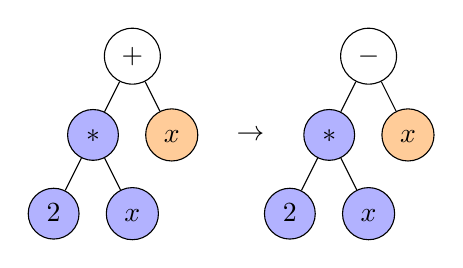
\begin{tikzpicture}
    \node[varnode] (del_plus) {$+$};
    \node[varnode, colorA] (del_times) at ($(del_plus)+(-0.5,-1)$) {$*$};
    \node[varnode, colorB] (del_one) at ($(del_plus)+(0.5,-1)$) {$x$};
    \node[varnode, colorA] (del_two) at ($(del_times)+(-0.5,-1)$) {$2$};
    \node[varnode, colorA] (del_three) at ($(del_times)+(0.5,-1)$) {$x$};
    \draw (del_plus) -- (del_times);
    \draw (del_plus) -- (del_one);
    \draw (del_times) -- (del_two);
    \draw (del_times) -- (del_three);

    \node[varnode] (ins_minus) at ($(del_plus)+(3,0)$) {$-$};
    \node[varnode, colorA] (ins_times) at ($(ins_minus)+(-0.5,-1)$) {$*$};
    \node[varnode, colorB] (ins_one) at ($(ins_minus)+(0.5,-1)$) {$x$};
    \node[varnode, colorA] (ins_two) at ($(ins_times)+(-0.5,-1)$) {$2$};
    \node[varnode, colorA] (ins_three) at ($(ins_times)+(0.5,-1)$) {$x$};
    \draw (ins_minus) -- (ins_times);
    \draw (ins_minus) -- (ins_one);
    \draw (ins_times) -- (ins_two);
    \draw (ins_times) -- (ins_three);

    \node (arrow) at ($(del_one)!0.5!(ins_times)$) {$\rightarrow$};
\end{tikzpicture}
\end{minipage}\hfill
\begin{minipage}{0.49\textwidth}
\centering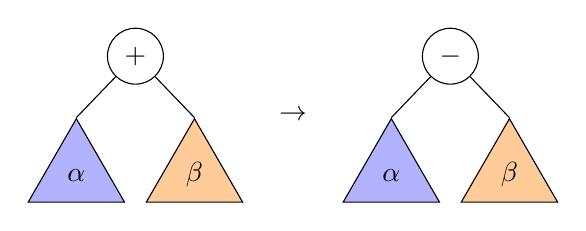
\begin{tikzpicture}
    \node[varnode] (del_plus) {$+$};
    \node[mvnode, colorA] (del_alpha) at ($(del_plus)+(-0.75,-1.5)$) {$\alpha$};
    \node[mvnode, colorB] (del_beta) at ($(del_plus)+(0.75,-1.5)$) {$\beta$};
    \draw (del_plus) -- (del_alpha.north);
    \draw (del_plus) -- (del_beta.north);

    \node[varnode] (ins_minus) at ($(del_plus)+(4,0)$) {$-$};
    \node[mvnode, colorA] (ins_alpha) at ($(ins_minus)+(-0.75,-1.5)$) {$\alpha$};
    \node[mvnode, colorB] (ins_beta) at ($(ins_minus)+(0.75,-1.5)$) {$\beta$};
    \draw (ins_minus) -- (ins_alpha.north);
    \draw (ins_minus) -- (ins_beta.north);

    \node (arrow) at ($($(del_beta)!0.5!(del_plus)$)!0.5!($(ins_alpha)!0.5!(ins_minus)$)$) {$\rightarrow$};
\end{tikzpicture}
\end{minipage}
\label{fig:metavar_elision}
\caption{The change $\change{(2*x)+x}{(2*x)-x}$ becomes $\change{\alpha+\beta} {\alpha-\beta}$ after meta-variable elision.}
\end{figure}

Trying to merge together two nodes in the AST is easy, we simply need
to check if they use the same root constructor, recursively merge if
it is the case, and fail otherwise. \yrg{Do you really ``fail''? I
  guess that you are just stopping the merging process when the two
  constructors differ.}

However, this approach is really bad with sequences ({\it e.g.}
sequences of functions or sequences of statements). Indeed, we do not
want to fully split a list~\yrg{You should explain what you mean by
  ``splitting'' a list.}  if only one element has been inserted,
removed or changed. Therefore, we use \yrg{...a refinement of
  standard...}  sequence edit scripts \yrg{ref?} instead as the output
of a merge operation on two sequences. We call ``spine'' the merged
part of the difference tree. Figure~\ref{fig:spine_seq_align} gives
an example of such spine.

\begin{figure}[ht]
\begin{minipage}{0.49\textwidth}
\centering\begin{tikzpicture}
    \node[varnode, colorDel] (del_block) {$\{\ldots\}$};
    \node[varnode, colorDel] (del_stmt1) at ($(del_block)+(-1,-1)$) {$\textbf{let}$};
    \node[varnode, colorDel] (del_stmt2) at ($(del_block)+(1,-1)$) {$=$};
    \node[varnode, colorDel] (del_x) at ($(del_stmt1)+(-0.5,-1)$) {$x$};
    \node[varnode, colorDel] (del_three) at ($(del_stmt1)+(0.5,-1)$) {$3$};
    \node[varnode, colorDel] (del_y) at ($(del_stmt2)+(-0.5,-1)$) {$y$};
    \node[varnode, colorDel] (del_yx) at ($(del_stmt2)+(0.5,-1)$) {$x$};
    \draw (del_block) -- (del_stmt1);
    \draw (del_block) -- (del_stmt2);
    \draw (del_stmt1) -- (del_x);
    \draw (del_stmt1) -- (del_three);
    \draw (del_stmt2) -- (del_y);
    \draw (del_stmt2) -- (del_yx);

    \node[varnode, colorIns] (ins_block) at ($(del_plus)+(4.1,0)$) {$\{\ldots\}$};
    \node[varnode, colorIns] (ins_stmt1) at ($(ins_block)+(-1,-1)$) {$=$};
    \node[varnode, colorIns] (ins_stmt2) at ($(ins_block)+(1,-1)$) {$=$};
    \node[varnode, colorIns] (ins_y) at ($(ins_stmt1)+(-0.5,-1)$) {$y$};
    \node[varnode, colorIns] (ins_five) at ($(ins_stmt1)+(0.5,-1)$) {$5$};
    \node[varnode, colorIns] (ins_z) at ($(ins_stmt2)+(-0.5,-1)$) {$z$};
    \node[varnode, colorIns] (ins_nine) at ($(ins_stmt2)+(0.5,-1)$) {$9$};
    \draw (ins_block) -- (ins_stmt1);
    \draw (ins_block) -- (ins_stmt2);
    \draw (ins_stmt1) -- (ins_y);
    \draw (ins_stmt1) -- (ins_five);
    \draw (ins_stmt2) -- (ins_z);
    \draw (ins_stmt2) -- (ins_nine);

    \node (arrow) at ($(del_stmt2)!0.5!(ins_stmt1)$) {$\rightarrow$};
\end{tikzpicture}
\end{minipage}\hfill
\begin{minipage}{0.45\textwidth}
\centering\begin{tikzpicture}
    \node[varnode] (spine_block) {$\{\ldots\}$};
    \node[changenode, colorDel] (spine_stmt1) at ($(spine_block)+(-2.5,-1.5)$) {\tikz{
        \node[varnode] (del_stmt) {$\textbf{let}$};
        \node[varnode] (del_x) at ($(del_stmt)+(-0.5,-1)$) {$x$};
        \node[varnode] (del_three) at ($(del_stmt)+(0.5,-1)$) {$3$};
        \draw (del_stmt) -- (del_x);
        \draw (del_stmt) -- (del_three);
    }};
    \node[varnode] (spine_stmt2) at ($(spine_block)+(-0.25,-1)$) {$=$};
    \node[changenode, colorIns] (spine_stmt3) at ($(spine_block)+(2.5,-1.5)$) {\tikz{
        \node[varnode] (ins_stmt) at ($(ins_block)+(1,-1)$) {$=$};
        \node[varnode] (ins_z) at ($(ins_stmt)+(-0.5,-1)$) {$z$};
        \node[varnode] (ins_nine) at ($(ins_stmt)+(0.5,-1)$) {$9$};
        \draw (ins_stmt) -- (ins_z);
        \draw (ins_stmt) -- (ins_nine);
    }};{};
    \node[varnode] (spine_y) at ($(spine_stmt2)+(-0.75,-1)$) {$y$};
    \node[changenode] (change_y) at ($(spine_stmt2)+(0.75,-1)$) {\tikz{
        \node[varnode, colorDel] (x) {$x$};
        \node[varnode, colorIns] (five) at ($(x)+(1.2,0)$) {$5$};
        \node (arrow) at ($(x)!0.5!(five)$) {$\rightarrow$};
    }};
    \draw (spine_block) -- (spine_stmt1);
    \draw (spine_block) -- (spine_stmt2);
    \draw (spine_block) -- (spine_stmt3);
    \draw (spine_stmt2) -- (spine_y);
    \draw (spine_stmt2) -- (change_y);
\end{tikzpicture}
\end{minipage}
\label{fig:spine_seq_align}
\caption{The change $\change{\{ \mathbf{let}\ x=3; y=x\}}{\{ y=5; z=9 \}}$ becomes $\{\mathst{\mathbf{let}\ x=3;}\ y = \change{x}{5}; \mathul{z = 9}\}$ after spine merging and sequence alignment.}
\end{figure}

The notion of syntactic differences and common spine are generic with
respect to the actual syntax of the source language. For this reason,
our formal definition for the difference language is parameterized
with respect to the source language grammar.  Therefore, we write
$S(\overrightarrow{t}, \overrightarrow{s})$ for a constructor from the
source language AST, with an arbitrary but fixed number of subtrees
($t$) and subsequences ($s$). For instance, one of the possible $S$
could be the language construction for conditional expression
%
\lstinline[mathescape]|if $t_{cond}$ { $\overrightarrow{s_{true}}$ } else { $\overrightarrow{s_{false}}$ }|%
with one expression sub-tree and two nested sequences of instructions.

This gives the following grammar for difference trees:
\begin{align*}
c &::= S(\overrightarrow{c}, \overrightarrow{c}) \typsep \alpha\\
t &::= S(\overrightarrow{t}, \overrightarrow{s}) \typsep \id \typsep \change{c}{c}\\
s &::= t \typsep \mathst{c} \typsep \mathul{c}\\
\end{align*}

\yrg{You must explain which language is supposed to be represented
by each nonterminal: $c$ is for code? $t$ for difference? $s$ for ?
It is not even clear to me...
}

Here $\id$ represents a hole for unchanged sub-tree, \st{strike
  through} represents deleted code, and \ul{underline} represents
inserted code.~\yrg{Notice that you already used this notation
before its introduction...}

\subsubsection{Computing a syntactic difference}

To compute a syntactic difference, we take ASTs of both the original
program and the modified program and we run the following algorithm:

\begin{enumerate}
  \item Compute a hash for each node of each AST.

  \item Take the subset of hashes occurring both in original and
    modified AST.

  \item Elide the nodes with a hash in the subset to remember just
    their hash.

  \item If an elided node does not match an elision with the same hash
    in the other tree, replace it by the original sub-tree.

  \item Merge both AST into a common spine where possible, else keep
    changes as two separate elided trees. Always try to align
    sequences using recursively a dynamic algorithm minimizing the
    number of nodes of the resulting tree.

  \item Replace each hash by a meta-variable letter (just an index in
    code), and replace changes $\change{\alpha}{\alpha}$ by $\id$ when
    $\alpha$ does not occur elsewhere.
\end{enumerate}

This algorithm is in $O(nm)$ where $n$ (resp. $m$) is the number of
node of the original (resp. modified) tree. The most computationally
expansive part of the algorithm is computing sequence alignments, all
the rest is linear.

\yrg{This description is too short given that this algorithm is one of
  your contributions. You should at least comment each step to explain
  its purpose and give (informal) arguments to convince the reader of
  the algorithm correctness.}

\subsubsection{Applying syntactic differences}

We can see syntactic differences as partial functions turning a syntax
tree into another syntax tree.  The difference between $d$ and $i$ is
therefore a function that is at least mapping $d$ to $i$, but it is
also defined on some other trees sharing all the relevant structure
with $d$.

The implied function of a difference tree is defined as follows: let
us suppose that we have $\Gamma$ a function from meta-variable
(occurring in the difference tree) to syntax trees, given by an
oracle. In practice, $\Gamma$ is constrained enough to be
inferred. \yrg{The previous points about $\Gamma$ really need
more explanations, otherwise the function seems a bit too ``magic''. You must
at least provide a forward pointer to a section describing how
you compute $\Gamma$.}
Then apply the following syntax-driven rules:
\yrg{Before the rules, we need a description of the judgment
and how to read it. As far as I understand the rules, there are
several judgments here... Besides, the syntax $... :: ...$ is
undefined if I am following correctly. Finally, it would be
more pedagogical to take each rule, to read it for the
reader and to comment them to convey an intuition about its
role. Notice that the notation with the vector of judgments
is not standard and will probably make the reviewers a bit
puzzled... You should probably use indices and universal
quantifications instead.}

\noindent
\begin{minipage}{.49\textwidth}
\begin{prooftree}
 \AxiomC{}
 \RightLabel{\textsc{Id}}
 \UnaryInfC{$\Gamma \vdash \id(t) = t$}
\end{prooftree}

\begin{prooftree}
 \AxiomC{$\Gamma \vdash d(t)$}
 \RightLabel{\textsc{Change}}
 \UnaryInfC{$\Gamma \vdash (\change{d}{i})(t) = \Gamma(i)$}
\end{prooftree}

\begin{prooftree}
 \AxiomC{$\overrightarrow{\Gamma \vdash t(d_t) = i_t}$}
 \AxiomC{$\overrightarrow{\Gamma \vdash s(d_s) = i_s}$}
 \RightLabel{\textsc{Spine}}
 \BinaryInfC{$\Gamma \vdash S(\overrightarrow{t},\overrightarrow{s})(S(\overrightarrow{d_t},\overrightarrow{d_s})) = S(\overrightarrow{i_t}, \overrightarrow{i_s})$}
\end{prooftree}

\begin{prooftree}
 \AxiomC{$\Gamma \vdash t(d) = i$}
 \AxiomC{$\Gamma \vdash r(d_r) = i_r$}
 \RightLabel{\textsc{SeqZip}}
 \BinaryInfC{$\Gamma \vdash (t::r)(d::d_r) = i::i_r$}
\end{prooftree}
\end{minipage}
\begin{minipage}{.49\textwidth}
\begin{prooftree}
 \AxiomC{$\Gamma \vdash c(d)$}
 \AxiomC{$\Gamma \vdash r(d_r) = i_r$}
 \RightLabel{\textsc{SeqDel}}
 \BinaryInfC{$\Gamma \vdash (\mathst{c}::r)(d::d_r) = i_r$}
\end{prooftree}

\begin{prooftree}
 \AxiomC{$\Gamma \vdash r(d_r) = i_r$}
 \RightLabel{\textsc{SeqIns}}
 \UnaryInfC{$\Gamma \vdash (\mathul{c}::r)(d_r) = \Gamma(c) :: i_r$}
\end{prooftree}

\begin{prooftree}
 \AxiomC{$\Gamma(\alpha) = d$}
 \RightLabel{\textsc{DelMv}}
 \UnaryInfC{$\Gamma \vdash \alpha(d)$}
\end{prooftree}

\begin{prooftree}
 \AxiomC{$\overrightarrow{\Gamma \vdash c_t(d_t)}$}
 \AxiomC{$\overrightarrow{\Gamma \vdash c_s(d_s)}$}
 \RightLabel{\textsc{DelSyn}}
 \BinaryInfC{$\Gamma \vdash S(\overrightarrow{c_t}, \overrightarrow{c_s})(S(\overrightarrow{d_t}, \overrightarrow{d_s}))$}
\end{prooftree}
\end{minipage}

\subsubsection{Practical considerations: how to extend a syntax tree}
Implementing an algorithm that requires extending a syntax tree can be
tidious in practice because we want to attach new information and/or
create holes on a fixed structure while keeping the typedness of the
tree.

Along this paper, I give a Rust implementation for the syntax
difference and merging algorithm of Rust programs. The parser used
(the syn\yrg{Ref?} crate) uses more than 180 types in its syntax
trees, so manual extension was not an option.

The solution I give is based on a somehow generic code generation
system (implemented as a procedural macro). The idea is that we want
to add the ability to extend a type family of mutually recursive sum
of products (nested enums and structs in Rust terminology) by
systematically changing some types with others, thus generating a new
family variant. Then, we also make a code generator to traverse or
convert between variants of the same family. After generation, manual
code is only required for the new structures of the trees. \yrg{What
  do you mean by ``the new structures of the trees''?}

\begin{lstlisting}[label=lst:codegen, caption={Usage example of the code generator for creating the hash-tagged family variant}]
syn_codegen! {
    pub mod hash {
        use crate::family_traits::Convert;
        use crate::hash_tree::{HashTagged, TreeHasher};

        #[derive(Hash, Eq, PartialEq)]
        extend_family! {
            Expr as HashTagged<Expr>,
            Vec<Stmt> as Vec<HashTagged<Stmt>>,
            Vec<Item> as Vec<HashTagged<Item>>,
            [...] // other type replacements
        }

        family_impl!(Convert<syn, self> for TreeHasher);
    }

    [...] // other family variants
}
\end{lstlisting}

\yrg{Please explain/comment this code snippet!}

\yrg{Please give an URL to get this crate.}

Note that for having a production ready tool, the current parser is
not adapted, as it systematically forgets the comments inside source
code. But this is left for future work as a pure engineering problem.

\subsection{Awareness colors}

Before merging differences together, we want to define a way of
keeping track of which commit introduced each modification. For that
we use a notion of awareness colors.

Each commit in a fusion gets an associated tint. If we denote by
$\mathbb{T}$ the set of all tints considered, we can define the color
set as $\mathbb{C} = \mathcal{P}(\mathbb{T})$. This forms the complete
lattice $(\mathbb{C}, \cup, \cap, \subset)$. We name the maximum in
this lattice white (equal to $\mathbb{T}$, denoted by $\top$) and the
minimum black (equal to $\emptyset$, denoted by $\bot$).

A modification~\yrg{Is ``modification'' as synonymous for ``commit''?
  for ``difference''?} gets the color $c \in \mathbb{C}$, if for all
tint in $c$, the associated commit is aware of the presence of the
colored source code.~\yrg{Presence where?} \yrg{You already
used $c$ in the syntax for differences!}

The white color having all the tints, it represents a consensus of all
the commits. On the other side, black represents the fact that no
single commit can claim responsibility for a given value. This makes
the white color the good choice for everything already present in the
original program, and black a color that we want to track and
avoid.\yrg{that is, a good color for conflitcs?}

Both code and modification can carry colors. Code has the color of the
commits that introduced it, or is white if it comes from the original
program. The same code can be introduced twice if the exact same
insertion has been done by multiple commits. In this case it will have
the union of both tints as its color. Similarly, insertions and
deletions have the color of all the commits that made them.

Before merging, we apply the singleton color corresponding to the
commit on the difference tree, recursively as follows:
\begin{align*}
{\color{red}c} &= {\color{red}S(\overrightarrow{c}, \overrightarrow{c})} \typsep \alpha\\
{\color{red}t} &= S(\overrightarrow{\color{red}t}, \overrightarrow{\color{red}s}) \typsep \id \typsep {\setstcolor{red}\setulcolor{red}\change{c}{\color{red}c}}\\
{\color{red}s} &= {\color{red}t} \typsep {\setstcolor{red}\mathst{c}} \typsep {\color{red}\mathul{c}}\\
\end{align*}

\yrg{Hmm, what is the formal meaning of these red terms? That's not
  standard to use colored terms. You should take some time to explain
  these colored notations. In my opinion, they are elegant but it
  takes some time to understand how to interpret them. In particular,
  it is not clear how a term can have several colors using that
  notation.}

Note that meta-variables and holes are never colored, and that AST
structures are not colored in the spine but are in the inserted
sub-trees. This reflects the fact that in the spine and inside holes,
code comes from the original source code, while elsewhere it is
introduced by the commit. \yrg{You should add a footnote saying that
the terms are not written in white for obvious practical reasons.
This raises the question: how do you write black (conflicted) terms?
I am wondering if you should not use the background color to colorize
terms...
}

\subsection{Merging differences}
Now that we have difference trees for each individual concurrent
change, we can try to merge them in a way that keeps track of the
origin of each piece of code.

\yrg{At this point, you must discuss what a merging algorithm is, why
  it is necessarily arbitrary (semantically speaking), and what are
  the design principles that guided your work to get a form of
  syntactical merge which seems to take no arbitrary choice at the
  level of syntax...}

However, as with line based merge, this merging operation can and will
regularly fail if someone wants to merge syntactically incompatible
changes.

We therefore break the symmetry between deletion and insertion trees
as there will be only one deletion and multiple insertions, and we
need to extend our difference types to accumulate potential conflicts.
\yrg{The logical implication is mysterious. You should explain in
more depth why we need to break the symmetry here.}

\begin{align*}
d &::= S(\overrightarrow{d}, \overrightarrow{d}) \typsep \alpha \typsep \MvConflict(\alpha, d, i) \\
i &::= S(\overrightarrow{i}, \overrightarrow{j}) \typsep \alpha \typsep \InsConflict(\overrightarrow{i})\\
j &::= i \typsep \DelConflict(i) \typsep \OrdConflict(\overrightarrow{i})\\
t &::= S(\overrightarrow{t}, \overrightarrow{s}) \typsep \id \typsep  \change{d}{i}\\
s &::= t \typsep \mathst{d} \typsep \DelConflict(d, i) \typsep \mathul{i} \typsep \OrdConflict(\overrightarrow{\overrightarrow{i}})\\
\end{align*}

\yrg{Take the time to explain the role of each nonterminal of this
grammar and to give an informal description of each syntactic
construction. It is impossible for a reader (and even for me) to
magically infer the semantics of all these constructions. You must
also explain how these types compare and interact with the previous types
for syntax differences.}

When dealing with meta-variables, that represent a multi-source
multi-target code move, our merging algorithm will try to push changes
toward the destination of the code movement.  This is done in a
two-phase way. First, if we have two changes facing each other we try
to inline one of them inside the deletion tree of the other, by
allowing differences wherever we have a meta-variable. To avoid making
any arbitrary choice, this is ignored if both changes could be inlined
in the other. Then, we check that these inlined changes are consistent
for each meta-variable, and if they are, we replace all occurrences of
the meta-variable by the obtained insertion.  \yrg{This paragraph is
  highly technical! You should probably start your explanations with
  simple cases and introduce these subtle situations afterwards.}

\begin{figure}[ht]
\begin{minipage}{0.49\textwidth}
\centering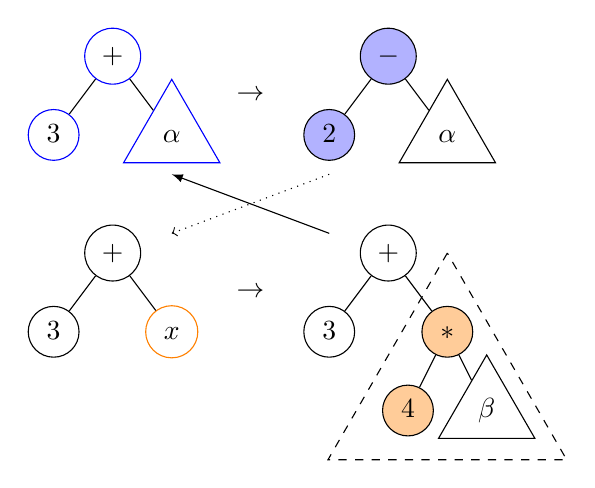
\begin{tikzpicture}
    \node[varnode, color=blue] (adel_plus) {$\color{black}+$};
    \node[varnode, color=blue] (adel_three) at ($(adel_plus)+(-0.75,-1)$) {$\color{black}3$};
    \node[mvnode, color=blue] (adel_alpha) at ($(adel_plus)+(0.75,-1)$) {$\color{black}\alpha$};
    \draw (adel_plus) -- (adel_three);
    \draw (adel_plus) -- (adel_alpha);

    \node[varnode, colorA] (ains_minus) at ($(adel_plus)+(3.5,0)$) {$-$};
    \node[varnode, colorA] (ains_two) at ($(ains_minus)+(-0.75,-1)$) {$2$};
    \node[mvnode] (ains_alpha) at ($(ains_minus)+(0.75,-1)$) {$\alpha$};
    \draw (ains_minus) -- (ains_two);
    \draw (ains_minus) -- (ains_alpha);

    \node (aarrow) at ($($(adel_alpha)!0.5!(adel_plus)$)!0.5!($(ains_two)!0.5!(ains_minus)$)$) {$\rightarrow$};
    
    \node[varnode] (bdel_plus) at ($(adel_plus)+(0,-2.5)$) {$+$};
    \node[varnode] (bdel_three) at ($(bdel_plus)+(-0.75,-1)$) {$3$};
    \node[varnode, color=orange] (bdel_x) at ($(bdel_plus)+(0.75,-1)$) {$\color{black}x$};
    \draw (bdel_plus) -- (bdel_three);
    \draw (bdel_plus) -- (bdel_x);

    \node[varnode] (bins_plus) at ($(bdel_plus)+(3.5,0)$) {$+$};
    \node[varnode] (bins_three) at ($(bins_plus)+(-0.75,-1)$) {$3$};
    \node[varnode, colorB] (bins_times) at ($(bins_plus)+(0.75,-1)$) {$*$};
    \node[varnode, colorB] (bins_four) at ($(bins_times)+(-0.5,-1)$) {$4$};
    \node[mvnode] (bins_beta) at ($(bins_times)+(0.5,-1)$) {$\beta$};
    \node[mvnode, dashed, minimum size=3.5cm] (bins_alpha) at ($(bins_times)+(0,-0.75)$) {};
    \draw (bins_plus) -- (bins_three);
    \draw (bins_plus) -- (bins_times);
    \draw (bins_times) -- (bins_four);
    \draw (bins_times) -- (bins_beta);
    
    \node (barrow) at ($($(bdel_x)!0.5!(bdel_plus)$)!0.5!($(bins_three)!0.5!(bins_plus)$)$) {$\rightarrow$};
    
    \draw[>=latex,->] ($(bins_plus)+(-0.75, 0.25)$) -- ($(adel_alpha)+(0, -0.5)$);
    \draw[->,dotted] ($(ains_two)+(0, -0.5)$) -- ($(bdel_plus)+(0.75, 0.25)$);
\end{tikzpicture}
\end{minipage}\hfill
\begin{minipage}{0.49\textwidth}
\centering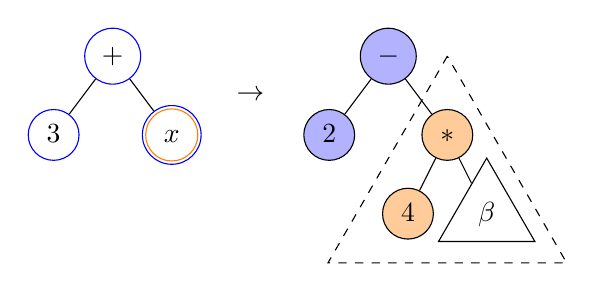
\begin{tikzpicture}
    \node[varnode, color=blue] (del_plus) {$\color{black}+$};
    \node[varnode, color=blue] (del_three) at ($(del_plus)+(-0.75,-1)$) {$\color{black}3$};
    \node[varnode, color=orange] (del_x) at ($(del_plus)+(0.75,-1)$) {$\color{black}x$};
    \node[varnode, color=blue] (del_x_out) at (del_x) {\phantom{M}};
    \draw (del_plus) -- (del_three);
    \draw (del_plus) -- (del_x_out);

    \node[varnode, colorA] (ins_minus) at ($(del_plus)+(3.5,0)$) {$-$};
    \node[varnode, colorA] (ins_two) at ($(ins_minus)+(-0.75,-1)$) {$2$};
    \node[varnode, colorB] (ins_times) at ($(ins_minus)+(0.75,-1)$) {$*$};
    \node[varnode, colorB] (ins_four) at ($(ins_times)+(-0.5,-1)$) {$4$};
    \node[mvnode] (ins_beta) at ($(ins_times)+(0.5,-1)$) {$\beta$};
    \node[mvnode, dashed, minimum size=3.5cm] (ins_alpha) at ($(ins_times)+(0,-0.75)$) {};
    \draw (ins_minus) -- (ins_two);
    \draw (ins_minus) -- (ins_times);
    \draw (ins_times) -- (ins_four);
    \draw (ins_times) -- (ins_beta);

    \node (arrow) at ($($(del_x)!0.5!(del_plus)$)!0.5!($(ins_two)!0.5!(ins_minus)$)$) {$\rightarrow$};
\end{tikzpicture}
\end{minipage}
\label{fig:metavar_inlining}
\caption{Meta-variable inlining}
\end{figure}

\yrg{The next paragraphs should probably come earlier, right after the
  syntax definitions... You should add a bit more structure to this
  section. I suggest: (a) what is a merging algorithm? (b) what is its
  high-level specification (input/output types, pre/post-conditions)?
  (c) what are the main design principles of your implementation?}

In absence of conflicts, merged differences have the same semantics as
simple difference trees.

Conflict represent parts that couldn't be merged and therefore prevent application of the difference on any tree. They can come from four different sources:
\begin{itemize}
  \item Insertion conflict ($\InsConflict$) simply represent two different insertions that were in the same place.
  \item Deletion conflict ($\DelConflict$) appears where one commit deletes a node while the other one had changes in it.
  \item Insert order conflict ($\OrdConflict$) is caused by two insertions taking place at the same location. As the merge operation is never performing any choice, it cannot arbitrarily order them.
  \item Meta-variable conflict ($\MvConflict$) is triggered when a meta-variable appears more than once in deletion tree, and the inlined insertions in each occurrences differ, therefore not giving a consistent replacement.
\end{itemize}

\subsubsection{Specification of the difference merging algorithm}

The difference merging algorithm is defined modulo two replacement
functions $\Gamma$ and $\Delta$ from meta-variables to respectively
insertion and deletion trees, that are heavily constrained and in
practice inferred during the merge.~\yrg{You should have forward
pointer to a section that precisely explains how this inference work.
You should also explain that this presentation (with oracles) simplifies
the formalization.}

\begin{prooftree}
 \AxiomC{$\Gamma, \Delta \vdash t_r \merge t_l = t$}
 \RightLabel{\textsc{Symmetry}}
 \UnaryInfC{$\Gamma, \Delta \vdash t_l \merge t_r = t$}
\end{prooftree}

\paragraph{Merge spine nodes}
\begin{prooftree}
 \AxiomC{}
 \RightLabel{\textsc{Id}}
 \UnaryInfC{$\Gamma, \Delta \vdash t \merge \id = \Delta(\Gamma(t))$}
\end{prooftree}

\begin{prooftree}
 \AxiomC{$\overrightarrow{\Gamma, \Delta \vdash t_l \merge t_r = t}$}
 \AxiomC{$\overrightarrow{\Gamma, \Delta \vdash s_l \merge s_r = s}$}
 \RightLabel{\textsc{Spine}}
 \BinaryInfC{$\Gamma, \Delta \vdash S(\overrightarrow{t_l}, \overrightarrow{s_l}) \merge S(\overrightarrow{t_r}, \overrightarrow{s_r}) = S(\overrightarrow{t}, \overrightarrow{s})$}
\end{prooftree}

\begin{prooftree}
 \AxiomC{$\Gamma \vdash i_l \not\subset d_r$}
 \AxiomC{$\Gamma \vdash i_r \not\subset d_l$}
 \AxiomC{$\Gamma \vdash d_l$}
 \AxiomC{$\Gamma \vdash d_r$}
 \RightLabel{\textsc{ChNoInl}}
 \QuaternaryInfC{$\Gamma, \Delta \vdash (\change{d_l}{i_l}) \merge (\change{d_r}{i_r}) = (\change{d_l \wedge d_r}{i_l \vee i_r})$}
\end{prooftree}

\begin{prooftree}
 \AxiomC{$\Gamma \vdash i_l \subset d_r = d'$}
 \AxiomC{$\Gamma \vdash i_r \not\subset d_l$}
 \AxiomC{$\Gamma \vdash d_l$}
 \RightLabel{\textsc{ChOneInl}}
 \TrinaryInfC{$\Gamma, \Delta \vdash (\change{d_l}{i_l}) \merge (\change{d_r}{i_r}) = (\change{d' \wedge d_l}{\Gamma(i_r)})$}
\end{prooftree}

\begin{prooftree}
 \AxiomC{$\Gamma \vdash i_l \subset d_r$}
 \AxiomC{$\Gamma \vdash i_r \subset d_l$}
 \AxiomC{$\Gamma \vdash d_l$}
 \AxiomC{$\Gamma \vdash d_r$}
 \RightLabel{\textsc{ChBothInl}}
 \QuaternaryInfC{$\Gamma, \Delta \vdash (\change{d_l}{i_l}) \merge (\change{d_r}{i_r}) = (\change{d_l \wedge d_r}{i_l \vee i_r})$}
\end{prooftree}

\paragraph{Merge sequence edit scripts (except insertions)}
\begin{prooftree}
 \AxiomC{$\Gamma, \Delta \vdash t_l \merge t_r = t$}
 \AxiomC{$\Gamma, \Delta \vdash r_l \merge r_r = r$}
 \RightLabel{\textsc{BothZip}}
 \BinaryInfC{$\Gamma, \Delta \vdash (t_l :: r_l) \merge (t_r :: r_r) = t :: r$}
\end{prooftree}

\begin{prooftree}
 \AxiomC{$\Gamma \vdash d_l$}
 \AxiomC{$\Gamma \vdash d_r$}
 \AxiomC{$\Gamma, \Delta \vdash r_l \merge r_r = r$}
 \RightLabel{\textsc{BothDel}}
 \TrinaryInfC{$\Gamma, \Delta \vdash (\mathst{d_l} :: r_l) \merge (\mathst{d_r} :: r_r) = \mathst{d_l \wedge d_r} :: r$}
\end{prooftree}

\begin{prooftree}
 \AxiomC{$t_r = \change{d_r}{i_r}$}
 \AxiomC{$\Gamma \vdash i_r \subset d_l = d'$}
 \AxiomC{$\Gamma \vdash d_r$}
 \AxiomC{$\Gamma, \Delta \vdash r_l \merge r_r = r$}
 \RightLabel{\textsc{DelZipInline}}
 \QuaternaryInfC{$\Gamma, \Delta \vdash (\mathst{d_l} :: r_l) \merge (t_r :: r_r) = \mathst{d' \wedge d_r} :: r$}
\end{prooftree}

\begin{prooftree}
 \AxiomC{$t_r = \change{d_r}{i_r}$}
 \AxiomC{$\Gamma \vdash i_r \not\subset d_l$}
 \AxiomC{$\Gamma \vdash d_l$}
 \AxiomC{$\Gamma \vdash d_r$}
 \AxiomC{$\Gamma, \Delta \vdash r_l \merge r_r = r$}
 \RightLabel{\textsc{DelZipConflict}}
 \QuinaryInfC{$\Gamma, \Delta \vdash (\mathst{d_l} :: r_l) \merge (t_r :: r_r) = \DelConflict(d_l \wedge d_r, \Gamma(i_r)) :: r$}
\end{prooftree}

\begin{prooftree}
 \AxiomC{$\Gamma \vdash i_l \not\subset d_r$}
 \AxiomC{$\Gamma \vdash i_r \not\subset d_l$}
 \AxiomC{$\Gamma \vdash d_l$}
 \AxiomC{$\Gamma \vdash d_r$}
 \AxiomC{$\Gamma, \Delta \vdash r_l \merge r_r = r$}
 \RightLabel{\textsc{DelConflNoInl}}
 \QuinaryInfC{$\Gamma, \Delta \vdash (\DelConflict(d_l, i_l) :: r_l) \merge (\DelConflict(d_r, i_r) :: r_r) = \DelConflict(d_l \wedge d_r, i_l \vee i_r) :: r$}
\end{prooftree}

\begin{prooftree}
 \AxiomC{$\Gamma \vdash i_l \subset d_r = d'_r$}
 \AxiomC{$\Gamma \vdash i_r \not\subset d_l$}
 \AxiomC{$\Gamma \vdash d_l$}
 \AxiomC{$\Gamma, \Delta \vdash r_l \merge r_r = r$}
 \RightLabel{\textsc{DelConflOneInl}}
 \QuaternaryInfC{$\Gamma, \Delta \vdash (\DelConflict(d_l, i_l) :: r_l) \merge (\DelConflict(d_r, i_r) :: r_r) = \DelConflict(d_l \wedge d'_r, \Gamma(i_r)) :: r$}
\end{prooftree}

\begin{prooftree}
 \AxiomC{$\Gamma \vdash i_l \subset d_r = d'_r$}
 \AxiomC{$\Gamma \vdash i_r \subset d_l = d'_l$}
 \AxiomC{$\Gamma, \Delta \vdash r_l \merge r_r = r$}
 \RightLabel{\textsc{DelConflBothInl}}
 \TrinaryInfC{$\Gamma, \Delta \vdash (\DelConflict(d_l, i_l) :: r_l) \merge (\DelConflict(d_r, i_r) :: r_r) = \mathst{d'_l \wedge d'_r} :: r$}
\end{prooftree}

\begin{prooftree}
 \AxiomC{$t_r = \change{d_r}{i_r}$}
 \AxiomC{$\Gamma, \Delta \vdash (\DelConflict(d_l, i_l) :: r_l) \merge (\DelConflict(d_r, i_r) :: r_r) = r$}
 \RightLabel{\textsc{DelConflZip}}
 \BinaryInfC{$\Gamma, \Delta \vdash (\DelConflict(d_l, i_l) :: r_l) \merge (t_r :: r_r) = r$}
\end{prooftree}

\begin{prooftree}
 \AxiomC{$\Gamma \vdash i_l \not\subset d_r$}
 \AxiomC{$\Gamma \vdash d_r$}
 \AxiomC{$\Gamma \vdash d_l$}
 \AxiomC{$\Gamma, \Delta \vdash r_l \merge r_r = r$}
 \RightLabel{\textsc{DelConflDelNoInl}}
 \QuaternaryInfC{$\Gamma, \Delta \vdash (\DelConflict(d_l, i_l) :: r_l) \merge (\mathst{d_r} :: r_r) = \DelConflict(d_l \wedge d_r, \Gamma(i_l)) :: r$}
\end{prooftree}

\begin{prooftree}
 \AxiomC{$\Gamma \vdash i_l \subset d_r = d'_r$}
 \AxiomC{$\Gamma \vdash d_l$}
 \AxiomC{$\Gamma, \Delta \vdash r_l \merge r_r = r$}
 \RightLabel{\textsc{DelConflDelInl}}
 \TrinaryInfC{$\Gamma, \Delta \vdash (\DelConflict(d_l, i_l) :: r_l) \merge (\mathst{d_r} :: r_r) = \mathst{d_l \wedge d'_r} :: r$}
\end{prooftree}

\paragraph{Merge insertions in sequence edit scripts}

\begin{prooftree}
 \AxiomC{$s_r \neq \mathul{\cdot}$}
 \AxiomC{$s_r \neq \OrdConflict(\cdot)$}
 \AxiomC{$\Gamma, \Delta \vdash r_l \merge (s_r :: r_r) = r$}
 \RightLabel{\textsc{InsBefore}}
 \TrinaryInfC{$\Gamma, \Delta \vdash (\mathul{i_l} :: r_l) \merge (s_r :: r_r) = \mathul{\Gamma(i_l)} :: r$}
\end{prooftree}

\begin{prooftree}
 \AxiomC{$\Gamma(i_l) = \Gamma(i_r) = i$}
 \AxiomC{$\Gamma, \Delta \vdash r_l \merge r_r = r$}
 \RightLabel{\textsc{InsSame}}
 \BinaryInfC{$\Gamma, \Delta \vdash (\mathul{i_l} :: r_l) \merge (\mathul{i_r} :: r_r) = \mathul{i} :: r$}
\end{prooftree}

\begin{prooftree}
 \AxiomC{$\Gamma, \Delta \vdash r_l \merge r_r = r$}
 \RightLabel{\textsc{OrdConfl}}
 \UnaryInfC{$\Gamma, \Delta \vdash (\mathul{i_l} :: r_l) \merge (\mathul{i_r} :: r_r) = \OrdConflict([\Gamma(i_l), \Gamma(i_r)]) :: r$}
\end{prooftree}

\begin{prooftree}
 \AxiomC{$s_r \neq \mathul{\cdot}$}
 \AxiomC{$s_r \neq \OrdConflict(\cdot)$}
 \AxiomC{$\Gamma, \Delta \vdash r_l \merge (s_r :: r_r) = r$}
 \RightLabel{\textsc{OrdConflBefore}}
 \TrinaryInfC{$\Gamma, \Delta \vdash (\OrdConflict(i_l) :: r_l) \merge (s_r :: r_r) = \OrdConflict(\Gamma(i_l)) :: r$}
\end{prooftree}

\begin{prooftree}
 \AxiomC{$\Gamma, \Delta \vdash r_l \merge r_r = r$}
 \RightLabel{\textsc{OrdConflPush}}
 \UnaryInfC{$\Gamma, \Delta \vdash (\mathul{i_l} :: r_l) \merge (\OrdConflict(i_r) :: r_r) = \OrdConflict(\Gamma(i_l) :: \Gamma(i_r)) :: r$}
\end{prooftree}

\begin{prooftree}
 \AxiomC{$\Gamma, \Delta \vdash r_l \merge r_r = r$}
 \RightLabel{\textsc{OrdConflMerge}}
 \UnaryInfC{$\Gamma, \Delta \vdash (\OrdConflict(i_l) :: r_l) \merge (\OrdConflict(i_r) :: r_r) = \OrdConflict(\Gamma(i_l) \mathbin{@} \Gamma(i_r)) :: r$}
\end{prooftree}

\paragraph{Inclusion of insertion inside a deletion}\phantom{ }

\noindent
\begin{minipage}{.49\textwidth}
\begin{prooftree}
 \AxiomC{$\overrightarrow{\Gamma \vdash i \subset d = d'}$}
 \RightLabel{\textsc{SynIncl}}
 \UnaryInfC{$\Gamma \vdash S(\overrightarrow{i}) \subset S(\overrightarrow{d}) = S(\overrightarrow{d'})$}
\end{prooftree}

\begin{prooftree}
 \AxiomC{$\Gamma(\alpha) = \Gamma(i)$}
 \RightLabel{\textsc{MvIncl}}
 \UnaryInfC{$\Gamma \vdash i \subset \alpha = \alpha$}
\end{prooftree}
\end{minipage}\hfill
\begin{minipage}{.49\textwidth}
\begin{prooftree}
 \AxiomC{$d \neq \alpha$}
 \AxiomC{$d \neq S(\cdot)$}
 \RightLabel{\textsc{SynNotIncl}}
 \BinaryInfC{$\Gamma \vdash S(\cdot) \not\subset d$}
\end{prooftree}

\begin{prooftree}
 \AxiomC{$d \neq \alpha$}
 \AxiomC{$i \neq S(\cdot)$}
 \RightLabel{\textsc{InsNotIncl}}
 \BinaryInfC{$\Gamma \vdash i \not\subset d$}
\end{prooftree}
\end{minipage}

\begin{prooftree}
 \AxiomC{$\Gamma(\alpha) = \top$}
 \RightLabel{\textsc{MvConfl}}
 \UnaryInfC{$\Gamma \vdash i \subset \alpha = \MvConflict(\alpha, \alpha, i)$}
\end{prooftree}

\begin{prooftree}
 \AxiomC{$\Gamma(\alpha) = \top$}
 \RightLabel{\textsc{MvConflPush}}
 \UnaryInfC{$\Gamma \vdash i \subset \MvConflict(\alpha, d, i') = \MvConflict(\alpha, d, i \vee i')$}
\end{prooftree}

\paragraph{Coherence with $\Gamma$ of kept deletion trees}\phantom{ }

\noindent\begin{minipage}{0.49\textwidth}
\begin{prooftree}
 \AxiomC{$\overrightarrow{\Gamma \vdash d}$}
 \RightLabel{\textsc{KeptSyn}}
 \UnaryInfC{$\Gamma \vdash S(\overrightarrow{d})$}
\end{prooftree}
\end{minipage}\hfill
\begin{minipage}{0.49\textwidth}
\begin{prooftree}
 \AxiomC{$\Gamma(\alpha) = \top$}
 \AxiomC{$\Gamma \vdash d$}
 \RightLabel{\textsc{KeptMvConfl}}
 \BinaryInfC{$\Gamma \vdash \MvConflict(\alpha, d, i)$}
\end{prooftree}
\end{minipage}

\begin{prooftree}
 \AxiomC{$\Gamma(\alpha) \in \{ \oplus(\Delta(\alpha)), \top \}$}
 \RightLabel{\textsc{KeptMv}}
 \UnaryInfC{$\Gamma \vdash \alpha$}
\end{prooftree}

Where $\oplus$ is a function transposing a deletion tree to an insertion tree by passing through each meta-variable conflict so that $\oplus(\MvConflict(\alpha, d, i)) = \oplus(d)$.

\paragraph{Deletion intersection}\phantom{ }

\noindent\begin{minipage}{0.49\textwidth}
\begin{prooftree}
 \AxiomC{$\overrightarrow{\Delta \vdash d_l \wedge d_r = d}$}
 \RightLabel{\textsc{SameSyn}}
 \UnaryInfC{$\Delta \vdash S^{c_l}(\overrightarrow{d_l}) \wedge S^{c_r}(\overrightarrow{d_r}) = S^{c_l \cup c_r}(\overrightarrow{d})$}
\end{prooftree}

\begin{prooftree}
 \AxiomC{}
 \RightLabel{\textsc{SameMv}}
 \UnaryInfC{$\Delta \vdash \alpha^{c_l} \wedge \alpha^{c_r} = \Delta(\alpha)^{c_l \cup c_r}$}
\end{prooftree}
\end{minipage}\hfill
\begin{minipage}{0.49\textwidth}
\begin{prooftree}
 \AxiomC{$\Delta \vdash \Delta(\alpha) \wedge d_r = \Delta(\alpha)$}
 \RightLabel{\textsc{MvLeft}}
 \UnaryInfC{$\Delta \vdash \alpha^{c_l} \wedge d_r^{c_r} = \Delta(\alpha)^{c_l \cup c_r}$}
\end{prooftree}

\begin{prooftree}
 \AxiomC{$\Delta \vdash \Delta(\alpha) \wedge d_l = \Delta(\alpha)$}
 \RightLabel{\textsc{MvRight}}
 \UnaryInfC{$\Delta \vdash d_l^{c_l} \wedge \alpha^{c_r} = \Delta(\alpha)^{c_l \cup c_r}$}
\end{prooftree}
\end{minipage}

\begin{prooftree}
 \AxiomC{$\Delta \vdash d_l \wedge d_r = d$}
 \RightLabel{\textsc{MvConflLeft}}
 \UnaryInfC{$\Delta \vdash \MvConflict(\alpha, d_l^{c_l}, i) \wedge d_r^{c_r} = \MvConflict(\alpha, d^{c_l \cup c_r}, \Gamma(i))$}
\end{prooftree}

\begin{prooftree}
 \AxiomC{$\Delta \vdash d_l \wedge d_r = d$}
 \RightLabel{\textsc{MvConflRight}}
 \UnaryInfC{$\Delta \vdash d_l^{c_l} \wedge \MvConflict(\alpha, d_r^{c_r}, i) = \MvConflict(\alpha, d^{c_l \cup c_r}, \Gamma(i))$}
\end{prooftree}

\paragraph{Simplification of insertion union}

\begin{prooftree}
 \AxiomC{$\Gamma(i_l)^{c_l} = \Gamma(i_r)^{c_r} = i$}
 \RightLabel{\textsc{SameIns}}
 \UnaryInfC{$\Gamma \vdash i_l \vee i_r = i^{c_l \cup c_r}$}
\end{prooftree}

\begin{prooftree}
 \AxiomC{$\overrightarrow{\Gamma \vdash i_l \vee i_r = i}$}
 \RightLabel{\textsc{InsSyn}}
 \UnaryInfC{$\Gamma \vdash S^{c_l}(\overrightarrow{i_l}) \vee S^{c_r}(\overrightarrow{i_r}) = S^{c_l \cup c_r}(\overrightarrow{i})$}
\end{prooftree}

\begin{prooftree}
 \AxiomC{}
 \RightLabel{\textsc{InsConfl}}
 \UnaryInfC{$\Gamma \vdash i_l \vee i_r = \InsConflict(\Gamma(i_l), \Gamma(i_r))$}
\end{prooftree}

\subsubsection{Algorithm for merging differences}
The above specification is telling what a merged version must look like but doesn't tell how to compute this merged version. Simply following the rules is not enough, because we have two global variables $\Gamma$ and $\Delta$ to infer. Moreover, for $\Gamma$ there is a priori several possibilities. Hopefully, we can easily distinguish one that will minimize the number of conflicts generated. We want a valid $\Gamma$ that minimize the number of meta-variables associated to $\top$.

From a high level point of view, the merging algorithm follows these steps:
\begin{itemize}
 \item Ensure that all the meta-variables used in both programs are disjoint by alpha-renaming whenever necessary.
 \item Align the spines of both difference trees. This requires unrolling whenever one of the difference tree still has a spine node while the other has a difference at the same place. This step also aligns the sequences and detect insert order conflicts.
 \begin{figure}[ht]
\begin{minipage}{0.33\textwidth}
\centering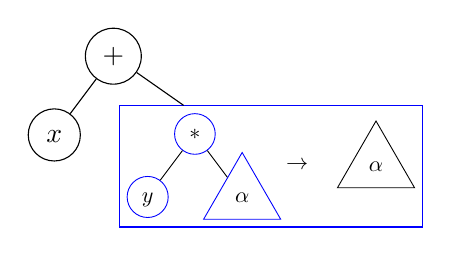
\begin{tikzpicture}
\node[varnode] (plus) {$+$};
\node[varnode] (x) at ($(plus)+(-0.75,-1)$) {$x$};
\node[changenode, color=blue] (change) at ($(plus)+(2,-1.4)$) {\tikz[color=black]{
    \node[varnode, color=blue] (del_times) {$\color{black}*$};
    \node[varnode, color=blue] (del_y) at ($(del_times)+(-0.75,-1)$) {$\color{black}y$};
    \node[mvnode, color=blue] (del_alpha) at ($(del_times)+(0.75,-1)$) {$\color{black}\alpha$};
    \draw (del_times) -- (del_y);
    \draw (del_times) -- (del_alpha);
    
    \node[mvnode] (ins_alpha) at ($(del_times)!0.5!(del_alpha)+(2.5, 0)$) {$\alpha$};
    \node (arrow) at ($(del_times)!0.5!(del_alpha)!0.5!(ins_alpha)$) {$\rightarrow$};
}};
\draw (plus) -- (x);
\draw (plus) -- (change);
\end{tikzpicture}
\end{minipage}\hfill
\begin{minipage}{0.33\textwidth}
\centering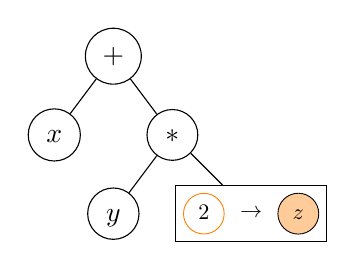
\begin{tikzpicture}
\node[varnode] (plus) {$+$};
\node[varnode] (x) at ($(plus)+(-0.75,-1)$) {$x$};
\node[varnode] (times) at ($(plus)+(0.75,-1)$) {$*$};
\node[varnode] (y) at ($(times)+(-0.75,-1)$) {$y$};
\node[changenode] (change) at ($(times)+(1,-1)$) {\tikz{
    \node[varnode, color=orange] (two) {$\color{black}2$};
    \node[varnode, colorB] (z) at ($(two)+(1.5, 0)$) {$z$};
    \node (arrow) at ($(two)!0.5!(z)$) {$\rightarrow$};
}};
\draw (plus) -- (x);
\draw (plus) -- (times);
\draw (times) -- (y);
\draw (times) -- (change);
\end{tikzpicture}
\end{minipage}
\hfill
\begin{minipage}{0.33\textwidth}
\centering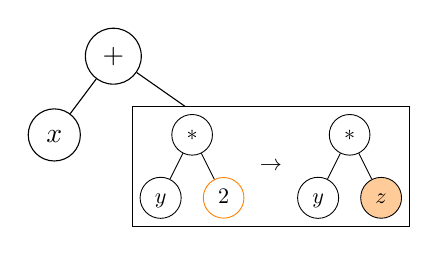
\begin{tikzpicture}
\node[varnode] (plus) {$+$};
\node[varnode] (x) at ($(plus)+(-0.75,-1)$) {$x$};
\node[changenode] (change) at ($(plus)+(2,-1.4)$) {\tikz{
    \node[varnode] (del_times) {$\color{black}*$};
    \node[varnode] (del_y) at ($(del_times)+(-0.5,-1)$) {$\color{black}y$};
    \node[varnode, color=orange] (del_two) at ($(del_times)+(0.5,-1)$) {$\color{black}2$};
    \draw (del_times) -- (del_y);
    \draw (del_times) -- (del_two);
    
    \node[varnode] (ins_times) at ($(del_times)+(2.5, 0)$) {$*$};
    \node[varnode] (ins_y) at ($(ins_times)+(-0.5,-1)$) {$y$};
    \node[varnode, colorB] (ins_z) at ($(ins_times)+(0.5,-1)$) {$z$};
    \draw (ins_times) -- (ins_y);
    \draw (ins_times) -- (ins_z);
    
    \node (arrow) at ($($(del_times)!0.5!(del_two)$)!0.5!($(ins_times)!0.5!(ins_y)$)$) {$\rightarrow$};
}};
\draw (plus) -- (x);
\draw (plus) -- (change);
\end{tikzpicture}
\end{minipage}
\label{fig:spine-alignment}
\caption{Spine alignment: We unwind the spine of the second tree producing the third in order to be aligned with first.}
\end{figure}
 \item Merge the insertion trees together. For each insertion we try to inline it inside the facing deletion tree first. If only one inlining could succeed, then we perform it, else we try to merge together the insertion trees. This take the union of tints as resulting color and create conflicts whenever both insertion do not match. By performing inlinings, we can remember $\Gamma^*$ a map form meta-variables to a list of the trees that were inlined on the metavariable.
 \item Merge the deletion trees together. For that, we build $\Delta$ as we merge the sub-trees.
 \item Then we perform all the substitutions wherever there are meta-variables with a replacement in $\Delta$ for deletion trees, and in $\Gamma$ for insertion trees.
\end{itemize}

If we want to merge more than two differences, we can reapply the same algorithm on already merged trees, thus accumulating modifications but also conflicts.

\subsection{Properties of the generated merged difference tree}
Despite the rather arbitrary choice of doing this specific syntactic merge, our algorithm provides some good properties.

\paragraph{Preserve common spine} All the nodes that are inside the spine of both commits are preserved.

\paragraph{Deletion tree intersection} If some code is deleted in one of the commits, it must also be deleted in the merged result colored with at least as many tints. Moreover, if two commits delete the same code, the result pushes meta-variables as far as possible down the tree.

\paragraph{Domain} First, we can notice that in absence of conflicts, the domain of the merged difference is the intersection of the domains of both inputs. Mathematically, we have: $\dom(t_1 \merge t_2) = \dom(t_1) \cap \dom(t_2)$. This comes from spine preservation combined with deletion tree intersection.

\paragraph{Idempotence} $t \merge t = t$. This comes from the fact that we do not let conflicts happen when both tree aggree on a common value. The property can be extended to differently colored tree as: $t^{c_1} \merge t^{c_2} = t^{c_1 \cup c_2}$.

\paragraph{Commutativity} $t_1 \merge t_2 = t_2 \merge t_1$, it comes from the symmetry in rules and shows that we cannot treat differently the left and the right commits, thus never favoring one side against the other. There is a little limitation though, we must consider that the order inside conflicts does not matter: $\InsConflict(i_1, i_2) = \InsConflict(i_2, i_1)$, $\OrdConflict([\overrightarrow{i}]) = \OrdConflict(\sigma[\overrightarrow{i}])$  for any permutation $\sigma$ and $\MvConflict(\alpha, \MvConflict(\beta, d, i_\beta), i_\alpha) = \MvConflict(\beta, \MvConflict(\alpha, d, i_\alpha), i_\beta)$.

\paragraph{Preserve introduced nodes} For all nodes that are introduced in one of the commits, we know that it will be found at least once in the merged result colored with at least as many tints. However, we cannot say anything about location of these introduced nodes because their code might have been displaced by metavariable inlining.

\paragraph{Compatible with composition} If $d \in \dom(t_1 \circ t_2)$, then if $t_1 \circ t_2 = t_2 \circ t_1$, we have $(t_1 \merge t_2)(d) = (t_1 \circ t_2)(d)$. Here the precondition will be true for differences without code moves. This means that on orthogonal changes, the merge operation is the same as the composition where they are both defined. \todo{Check that we cannot remove the domain assumption}

\paragraph{Compatible with inverse} If $d \in \dom(t_1^{-1} \circ (t_1 \merge t_2))$, then $(t_1^{-1} \circ (t_1 \merge t_2))(d) = t_2(d)$. Note here that inverse is defined for differences without colors, so the equality holds only after removing all colors from $t_1$ and $t_2$.


\section{Semantic merge}
\label{sec:semantic-merge}

Having two commits syntactically merged do not mean that the result is a valid semantic combination that respect the intentions of all original committers.

\begin{lstlisting}[label=lst:double-incr, caption={Double fix of the same function by different commits. The syntactic fusion does not create a conflict be semantically we can create a new bug here.}]
fn compute_something(x: i32) -> i32 {
    let mut a = x * x;
    @\color{blue}\ul{a += 1;}@
    @\setstcolor{orange}\st{a} $\rightarrow$ {\color{orange}\ul{a + 1}}@
}
\end{lstlisting}

That's why after the syntax merging step, we also want to check the semantic of the fusion.

In this section we will show that first non-conflicting difference trees can be interpreted as correlation oracles between the original code and a merged candidate. And secondly that we can derive a runtime analysis that ensures that there is no unresolved ambiguity introduced by the fusion operation. In future works, this runtime analysis could be refined into a static analysis.

If we combine this invariant with the fact that the fusion never lose any introduced change, we obtain the certainty that the intentions inside all original commits are respected, because both changes and implicit environment assumptions are preserved.

\subsection{Operational semantics of the studied language}
In this paper, we will use the following programming language, a simplified version of Rust. It has been chosen because it allows us to explore both functional and imperative coding styles, and we stripped all the borrowing and trait systems that could be difficult to understand for a reader without any Rust background.

\newcommand{\ident}{\mathbb{I}}
\newcommand{\typ}{\mathbb{T}}
Syntactically, with $\ident$ the set of variable and function identifiers, $\typ$ the set of type identifiers and $\diamond$ (resp. $\star$) the set of primitive binary (resp. unary) functions, it is defined by:
\begin{align*}
program &::= \boxed{item}^*\\
item &::= func \typsep enum\\
enum &::= \mathbf{enum}\ \typ\ \{ \boxed{\ident(\boxed{\typ,}^*),}^* \}\\
func &::= \mathbf{fn}\ \ident(\boxed{\ident: \typ}^*) \rightarrow \typ\ block\\
block &::= \{ \boxed{expr;}^* expr \}\\
expr &::= \ident \typsep literal \typsep \star expr \typsep expr \diamond expr \typsep \ident = expr \typsep \ident(\boxed{expr}^*) \typsep block\\
&\typsep \mathbf{if}\ expr\ block\ \mathbf{else}\ block \typsep \mathbf{while}\ expr\ block \typsep \mathbf{match}\ expr\ \{ \boxed{\ident(\boxed{\ident,}^*) \Rightarrow expr,}^* \}\\
&\typsep \mathbf{continue} \typsep \mathbf{break} \typsep \textbf{return}\ expr\\
literal &::= () \typsep \mathbf{true} \typsep \mathbf {false} \typsep \mathbb{Z}
\end{align*}

To define the semantics, we give the program state as a tuple $\rtstate{\kappa}{v}{S}$ where $\kappa$ is the continuation, $v$ the value of the last computed expression and $S$ the local store stack. For function calls, we can push a new store on the previous one, only the topmost store can be used and updated as it correspond to the current function.

We also keep the set of constructors, and the set of function as a global state. We denote $\mathbb{G}(f)$ the body of function $f$ taken from global state. Types do not play any role in reduction rules, but we will assume that programs are already well typed. The initial state is given by the call of the entry point function $f$ with its arguments $\overrightarrow{x_a}$: $\rtstate{\mathbb{G}(f)}{()}{\{\overrightarrow{x_a \leftarrow v_a}\}}$.

Then the program follows the reduction rules below:
\begin{align*}
\rtstate{\{\overrightarrow{stmt;}\ expr\} \cdot \kappa}{v}{S} &\rightarrow \rtstate{\overrightarrow{stmt} \cdot expr \cdot \kappa}{()}{S}\\
\rtstate{x = e \cdot \kappa}{v}{S} &\rightarrow \rtstate{e \cdot x = \square \cdot \kappa}{()}{S}\\
\rtstate{x = \square \cdot \kappa}{v}{S} &\rightarrow \rtstate{\kappa}{()}{S[x \leftarrow v]}\\
\rtstate{x \cdot \kappa}{v}{S} &\rightarrow \rtstate{\kappa}{S(x)}{S}\\
\rtstate{literal \cdot \kappa}{v}{S} &\rightarrow \rtstate{\kappa}{literal}{S}\\
\rtstate{\star e \cdot \kappa}{v}{S} &\rightarrow \rtstate{e \cdot \star \square \cdot \kappa}{()}{S}\\
\rtstate{\star \square \cdot \kappa}{v}{S} &\rightarrow \rtstate{\kappa}{\star v}{S}\\
\rtstate{e_1 \diamond e_2 \cdot \kappa}{v}{S} &\rightarrow \rtstate{e_1 \cdot \square \diamond e_2 \cdot \kappa}{()}{S}\\
\rtstate{\square \diamond e_2 \cdot \kappa}{v}{S} &\rightarrow \rtstate{e_2 \cdot v \diamond \square \cdot \kappa}{()}{S}\\
\rtstate{v_1 \diamond \square \cdot \kappa}{v_2}{S} &\rightarrow \rtstate{\kappa}{v_1 \diamond v_2}{S}\\
\rtstate{\varphi(\overrightarrow{v_a}, e, \overrightarrow{e_r}) \cdot \kappa}{v}{S} &\rightarrow \rtstate{e \cdot \varphi(\overrightarrow{v_a}, \square, \overrightarrow{e_r}) \cdot \kappa}{()}{S}\\
\rtstate{\varphi(\overrightarrow{v_a}, \square, \overrightarrow{e_r}) \cdot \kappa}{v}{S} &\rightarrow \rtstate{\varphi(\overrightarrow{v_a}, v, \overrightarrow{e_r}) \cdot \kappa}{()}{S}\\
\rtstate{f(\overrightarrow{v_a}) \cdot \kappa}{v}{S} &\rightarrow \rtstate{\mathbb{G}(f) \cdot \mathbf{eof} \cdot \kappa}{()}{\{\overrightarrow{a \leftarrow v_a}\} :: S}\\
\rtstate{C(\overrightarrow{v_a}) \cdot \kappa}{v}{S} &\rightarrow \rtstate{\kappa}{C(\overrightarrow{v_a})}{S}\\
\rtstate{\mathbf{if}\ e_{cond}\ b_{true}\ \mathbf{else}\ b_{false} \cdot  \kappa}{v}{S} &\rightarrow \rtstate{e_{cond} \cdot \mathbf{if}\ \square\ b_{true}\ \mathbf{else}\ b_{false} \cdot \kappa}{()}{S}\\
\rtstate{\mathbf{if}\ \square\ b_{true}\ \mathbf{else}\ b_{false} \cdot  \kappa}{\mathbf{true}}{S} &\rightarrow \rtstate{b_{true} \cdot \kappa}{()}{S}\\
\rtstate{\mathbf{if}\ \square\ b_{true}\ \mathbf{else}\ b_{false} \cdot  \kappa}{\mathbf{false}}{S} &\rightarrow \rtstate{b_{false} \cdot \kappa}{()}{S}\\
\rtstate{\mathbf{while}\ e_{cond}\ b \cdot \kappa}{v}{S} &\rightarrow \rtstate{\mathbf{if}\ e_{cond}\ \{ b;\ \mathbf{while}\ e_{cond}\ b \}\  \mathbf{else}\ \{\} \cdot \kappa}{()}{S}\\
\rtstate{\mathbf{match}\ e_{scrut}\ \{ \overrightarrow{C(\overrightarrow{x_C,}) \Rightarrow e_C,} \} \cdot \kappa}{v}{S} &\rightarrow \rtstate{e_{scrut} \cdot \mathbf{match}\ \square\ \{ \overrightarrow{C(\overrightarrow{x_C,}) \Rightarrow e_C,} \} \cdot \kappa}{()}{S}\\
\rtstate{\mathbf{match}\ \square\ \{ \overrightarrow{C(\overrightarrow{x_C,}) \Rightarrow e_C,} \} \cdot \kappa}{D(\overrightarrow{v_D})}{S} &\rightarrow \rtstate{e_D \cdot \kappa}{()}{S[\overrightarrow{x_D \leftarrow v_D}]}\\
\rtstate{\mathbf{continue} \cdot \overrightarrow{\kappa_{\neg while}} \cdot \textbf{while}\ e_{cond}\ b \cdot \kappa}{v}{S} &\rightarrow \rtstate{\textbf{while}\ e_{cond}\ b \cdot \kappa}{()}{S}\\
\rtstate{\mathbf{break} \cdot \overrightarrow{\kappa_{\neg while}} \cdot \textbf{while}\ e_{cond}\ b \cdot \kappa}{v}{S} &\rightarrow \rtstate{\kappa}{()}{S}\\
\rtstate{\mathbf{return}\ e \cdot \kappa}{v}{S} &\rightarrow \rtstate{e \cdot \mathbf{return}\ \square \cdot \kappa}{()}{S}\\
\rtstate{\mathbf{return}\ \square \cdot \overrightarrow{\kappa_{\neg eof}} \cdot \textbf{eof} \cdot \kappa}{v}{S} &\rightarrow \rtstate{\textbf{eof} \cdot \kappa}{v}{S}\\
\rtstate{\textbf{eof} \cdot \kappa}{v}{S_f :: S} &\rightarrow \rtstate{\kappa}{v}{S}\\
\end{align*}

\subsection{Definition of a correlation oracle}
\todo{Write this or maybe just quote T. Girka thesis}

\subsection{The colored difference oracle}
From this language and its semantics, we define what can be a correlation oracle that will be able to tell if a program trace exhibit an ambiguity created by the fusion.

We cannot do the verification directly on the merge candidate because we need to gather interferences created by deleted code.
\begin{lstlisting}[label=lst:del_interference, caption={Example of an ambiguity that would be missed if we don't analyze deleted code.}]
fn f() -> bool {
    let mut res = @\setstcolor{orange}\st{true} $\rightarrow$ {\color{orange}\ul{false}}@;
    @\setstcolor{blue}\st{res = !res;}@
    res
}
\end{lstlisting}

Therefore, in order to take into account the deleted code, we reason on both the original code known by all committers and the merge candidate. We then need to syncronize executions of these two programs and use the color algebra to verify that we do not have any unchecked ambiguity.

In general, synchronization between different programs is really hard but here we already have a good syntactic description of the differences between them. We can directly deduce the interleaving from the merged difference tree because it gives implicit correlation points. Indeed, each time there is a spine node that does not depend on the control flow decisions, we know for sure that both programs will at some point execute the same code, and we can syncronize this execution. Moreover, for each change, or divergent control flow decision, we know precisely  where it is located in the spine allowing to resyncronize easily when programs start to behave similarly again.

To express the interleaving between two programs, and compute the colors of the expressions, we use the correlation oracle framework defined above \todo{Check that it is indeed above}.

\begin{figure}[ht]
\begin{minipage}{.34\textwidth}
\begin{lstlisting}
fn f(c: bool) -> i32 {
    @\color{red}\st{let w = 40;}@
    let x = @\color{red}\st{2 + w}@ @$\rightarrow$@ @{\color{olive}\ul{42}}@;
    @\color{olive}\ul{let z = !c;}@
    let y = if @\color{red}\st{c}@ @$\rightarrow$@ @{\color{olive}\ul{z}}@ {
        @{\color{red}\st{2}} $\rightarrow$ {\color{olive}\ul{1}}@
    } else {
        @{\color{red}\st{x}} $\rightarrow$ {\color{olive}\ul{x * x}}@
    };
    x * y
}
\end{lstlisting}
\end{minipage}\hfill
\begin{minipage}{.65\textwidth}
\setstcolor{red}\setulcolor{olive}
\centering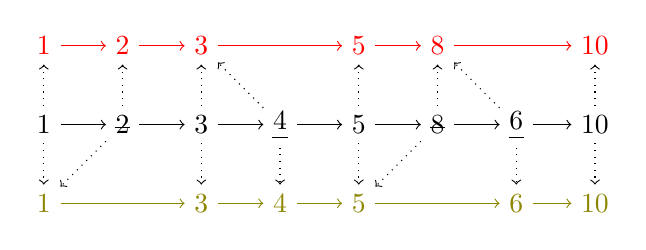
\begin{tikzpicture}
    \node (o1) {1};
    \node[right of=o1] (o2) {\st{2}};
    \node[right of=o2] (o3) {3};
    \node[right of=o3] (o4) {\ul{4}};
    \node[right of=o4] (o5) {5};
    \node[right of=o5] (o8) {\st{8}};
    \node[right of=o8] (o6) {\ul{6}};
    \node[right of=o6] (o10) {10};
    \draw[->] (o1) -- (o2);
    \draw[->] (o2) -- (o3);
    \draw[->] (o3) -- (o4);
    \draw[->] (o4) -- (o5);
    \draw[->] (o5) -- (o8);
    \draw[->] (o8) -- (o6);
    \draw[->] (o6) -- (o10);

    \node[red, above of=o1] (d1) {1};
    \node[red, above of=o2] (d2) {2};
    \node[red, above of=o3] (d3) {3};
    \node[red, above of=o5] (d5) {5};
    \node[red, above of=o8] (d8) {8};
    \node[red, above of=o10] (d10) {10};
    \draw[red, ->] (d1) -- (d2);
    \draw[red, ->] (d2) -- (d3);
    \draw[red, ->] (d3) -- (d5);
    \draw[red, ->] (d5) -- (d8);
    \draw[red, ->] (d8) -- (d10);
    \draw[dotted, ->] (o1) -- (d1);
    \draw[dotted, ->] (o2) -- (d2);
    \draw[dotted, ->] (o3) -- (d3);
    \draw[dotted, ->] (o4) -- (d3);
    \draw[dotted, ->] (o5) -- (d5);
    \draw[dotted, ->] (o8) -- (d8);
    \draw[dotted, ->] (o6) -- (d8);
    \draw[dotted, ->] (o10) -- (d10);

    \node[olive, below of=o1] (i1) {1};
    \node[olive, below of=o3] (i3) {3};
    \node[olive, below of=o4] (i4) {4};
    \node[olive, below of=o5] (i5) {5};
    \node[olive, below of=o6] (i6) {6};
    \node[olive, below of=o10] (i10) {10};
    \draw[olive, ->] (i1) -- (i3);
    \draw[olive, ->] (i3) -- (i4);
    \draw[olive, ->] (i4) -- (i5);
    \draw[olive, ->] (i5) -- (i6);
    \draw[olive, ->] (i6) -- (i10);
    \draw[dotted, ->] (o1) -- (i1);
    \draw[dotted, ->] (o2) -- (i1);
    \draw[dotted, ->] (o3) -- (i3);
    \draw[dotted, ->] (o4) -- (i4);
    \draw[dotted, ->] (o5) -- (i5);
    \draw[dotted, ->] (o8) -- (i5);
    \draw[dotted, ->] (o6) -- (i6);
    \draw[dotted, ->] (o10) -- (i10);
\end{tikzpicture}
\end{minipage}
\caption{Execution synchronization of a source and a destination program extracted from a difference tree without colors. For simplification, we show only one state for each line of code.}
\label{fig:oracle_sync_from_diff}
\end{figure}

Formally, the correlation oracle is defined as a program with a states that can be projected on either of the correlated programs. Moreover, it carries information about the co-execution of both programs.

Here we keep states as tuples $\rtstate{\kappa}{v}{S}$ but all the individual components are slightly more complex: $\kappa$ is the continuation but its elements can be either deleted (\st{$instr$}$^c$), inserted (\ul{$instr$}$^c$), or preserved ($instr$), depending on whether they occur on the original only, the merged candidate only or both. Deleted and inserted instructions carry a color with them. For each value $v$ or element of the store $S(x)$, they are replaced by a pair of values associated with a color $(v_{del}, v_{ins}, c)$.

The projection of a state to its equivalent in the original program $\pi_{del}$ removes all the inserted instructions in the continuation, and takes first elements of pairs of values, always ignoring colors. Same for the projection on the merge candidate $\pi_{ins}$, but removing deleted instructions, and taking second element inside pair of values.

For $S$ a store, we denote $S_{del} = \pi_{del} \circ S$, $S_{ins} = \pi_{ins} \circ S$ and $S_{c}$ the projection on the color of the value of $S$.

To describe how interleaving is done, we can also give operational semantic reductions.

In all the rules, if an instruction in the continuation should be both inserted and deleted according to the rules, it is simply discarded. If it should be deleted or inserted twice with different colors, we take the intersection of these colors.

\paragraph{Reusing rules from underlying language}
The rules from the underlying language can be reused for instructions that simply expand inside the continuation. In this case we preserve the deleted/inserted/preserved status and the color on the expansion.

For instance this gives the following reduction rules (non-exhaustive list):
\newbox\boxoverarrow
\sbox\boxoverarrow{$\overrightarrow{stmt;}$}
\begin{align*}
\rtstate{\mathst{\{{\usebox\boxoverarrow}\ expr\}}^k \cdot \kappa}{(v^-, v^+, c)}{S} &\rightarrow \rtstate{\overrightarrow{\mathst{stmt}}^k\cdot \mathst{expr}^k \cdot \kappa}{((), v^+, c)}{S}\\
\rtstate{\mathul{x = e}^k \cdot \kappa}{(v^-, v^+, c)}{S} &\rightarrow \rtstate{\mathul{e}^k \cdot \mathul{x = \square}^k \cdot \kappa}{(v^-, (), \top)}{S}\\
\rtstate{e_1 \diamond e_2 \cdot \kappa}{(v^-, v^+, c)}{S} &\rightarrow \rtstate{e_1 \cdot \square \diamond e_2 \cdot \kappa}{((), (), \top)}{S}\\
\end{align*}

\paragraph{Instruction producing value}
For instructions that change the current value, we need to be careful of the color of the result. There is three cases:
\begin{itemize}
  \item If the instruction is preserved, the output color is the intersection of the input colors
  \item If the instruction is deleted, the color of the value is tainted by the color of the deletion. However, the input values do not taint the result.
  \item If the instruction is inserted, the output color is the intersection of the input colors and the color of the insertion.
\end{itemize}

This leads to the following reduction rules:
\begin{align*}
\rtstate{x \cdot \kappa}{(v^-, v^+, c)}{S} &\rightarrow \rtstate{\kappa}{S(x)}{S}\\
\rtstate{\mathst{x}^k \cdot \kappa}{(v^-, v^+, c)}{S} &\rightarrow \rtstate{\kappa}{(S_{del}(x), v^+, c \cap k)}{S}\\
\rtstate{\mathul{x}^k \cdot \kappa}{(v^-, v^+, c)}{S} &\rightarrow \rtstate{\kappa}{(v^-, S_{ins}(x), S_c(x) \cap k)}{S}\\
\rtstate{literal \cdot \kappa}{(v^-, v^+, c)}{S} &\rightarrow \rtstate{\kappa}{(literal, literal, \top)}{S}\\
\rtstate{\mathst{literal}^k \cdot \kappa}{(v^-, v^+, c)}{S} &\rightarrow \rtstate{\kappa}{(literal, v^+, c \cap k)}{S}\\
\rtstate{\mathul{literal}^k \cdot \kappa}{(v^-, v^+, c)}{S} &\rightarrow \rtstate{\kappa}{(v^-, literal, k)}{S}\\
\rtstate{\star \square \cdot \kappa}{(v^-, v^+, c)}{S} &\rightarrow \rtstate{\kappa}{(\star v^-, \star v^+, c)}{S}\\
\rtstate{\mathst{\star \square}^k \cdot \kappa}{(v^-, v^+, c)}{S} &\rightarrow \rtstate{\kappa}{(\star v^-, v^+, c \cap k)}{S}\\
\rtstate{\mathul{\star \square}^k \cdot \kappa}{(v^-, v^+, c)}{S} &\rightarrow \rtstate{\kappa}{(v^-, \star v^+, c \cap k)}{S}\\
\rtstate{(v_l^-, v_l^+, c_l) \diamond \square \cdot \kappa}{(v_r^-, v_r^+, c_r)}{S} &\rightarrow \rtstate{\kappa}{(v_l^- \diamond v_r^-, v_l^+ \diamond v_r^+, c_l \cap c_r)}{S}\\
\rtstate{\mathst{(v_l^-, v_l^+, c_l) \diamond \square}^k \cdot \kappa}{(v_r^-, v^+, c)}{S} &\rightarrow \rtstate{\kappa}{(v_l^- \diamond v_r^-, v^+, c \cap k)}{S}\\
\rtstate{\mathul{(v_l^-, v_l^+, c_l) \diamond \square}^k \cdot \kappa}{(v^-, v_r^+, c_r)}{S} &\rightarrow \rtstate{\kappa}{(v^-, v_l^+ \diamond v_r^+, c_l \cap c_r \cap k)}{S}\\
\end{align*}

\paragraph{Assignment instructions}
With the same ideas as instruction producing a value, assignment instructions are treated as follows:
\begin{align*}
\rtstate{x = \square \cdot \kappa}{(v^-, v^+, c)}{S} &\rightarrow \rtstate{\kappa}{((), (), \top)}{S[x \leftarrow (v^-, v^+, c)]}\\
\rtstate{\mathst{x = \square}^k \cdot \kappa}{(v^-, v^+, c)}{S} &\rightarrow \rtstate{\kappa}{((), v^+, c \cap k)}{S[x \leftarrow (v^-, S_{ins}(x), S_c(x) \cap k)]}\\
\rtstate{\mathul{x = \square}^k \cdot \kappa}{(v^-, v^+, c)}{S} &\rightarrow \rtstate{\kappa}{(v^-, (), k)}{S[x \leftarrow (S_{del}(x), v^+, c \cap k)]}\\
\end{align*}

\paragraph{Function calls} Function calls do not need any special treatment, they can be considered as instructions simply expanding the function body into the continuation. The arguments keep their colors at the call point.
However note that $\mathbb{G}(f)$ potentially contains code that is either deleted or inserted.
\newbox\boxargs
\sbox\boxargs{$\overrightarrow{(v_a^-, v_a^+, c_a)}$}
\begin{align*}
\rtstate{f(\usebox\boxargs) \cdot \kappa}{(v^-, v^+, c)}{S} &\rightarrow \rtstate{\mathbb{G}(f) \cdot \mathbf{eof} \cdot \kappa}{((), (), \top)}{\{\overrightarrow{a \leftarrow (v_a^-, v_a^+, c_a)}\} :: S}\\
\rtstate{\mathst{f(\usebox\boxargs)}^k \cdot \kappa}{(v^-, v^+, c)}{S} &\rightarrow \rtstate{\mathst{\mathbb{G}(f)}^k \cdot \mathst{\mathbf{eof}}^k \cdot \kappa}{((), v^+, c \cap k)}{\{\overrightarrow{a \leftarrow (v_a^-, v_a^+, c_a)}\} :: S}\\
\rtstate{\mathul{f(\usebox\boxargs)}^k \cdot \kappa}{(v^-, v^+, c)}{S} &\rightarrow \rtstate{\mathul{\mathbb{G}(f)}^k \cdot \mathul{\mathbf{eof}}^k \cdot \kappa}{(v^-, (), k)}{\{\overrightarrow{a \leftarrow (v_a^-, v_a^+, c_a)}\} :: S}\\
\end{align*}
To make a static analysis, this function inlining approach might become too expansive and it might be replaced by some intraprocedural analysis.

\paragraph{Conditionals instructions} Conditional instruction are a bit harder to handle because they can split the execution between the correlated programs even when the branches themselves are totally in the spine. Indeed, both programs can show different value for the condition, and therefore take different paths. Also they could take the same value but only by chance and still be under the influence of some non-white color. In both case, we choose to split the execution and resyncronize only at the end of the branches.
\begin{align*}
\vrtstate{\mathbf{if}\ \square\ b_{true}\ \mathbf{else}\ b_{false} \cdot  \kappa}{(\mathbf{true}, \mathbf{true}, \top)}{S} &\rightarrow \vrtstate{b_{true} \cdot \kappa}{((), (), \top)}{S}\\
\vrtstate{\mathbf{if}\ \square\ b_{true}\ \mathbf{else}\ b_{false} \cdot  \kappa}{(\mathbf{false}, \mathbf{false}, \top)}{S} &\rightarrow \vrtstate{b_{false} \cdot \kappa}{((), (), \top)}{S}\\
\vrtstate{\mathbf{if}\ \square\ b_{true}\ \mathbf{else}\ b_{false} \cdot \kappa}{(v^-, v^+, c)}{S} &\rightarrow \vrtstate{\mathst{\mathbf{if}\ \square\ b_{true}\ \mathbf{else}\ b_{false}}^c \cdot \mathul{\mathbf{if}\ \square\ b_{true}\ \mathbf{else}\ b_{false}}^c \cdot \kappa}{((), (), \top)}{S}\\
\end{align*}

To reduce a conditional that is deleted, we can simply take the matching branch, but if it is inserted, we need to also take into account the color of the condition. This leads to these rules:
\begin{align*}
\rtstate{\mathst{\mathbf{if}\ \square\ b_{true}\ \mathbf{else}\ b_{false}}^k \cdot  \kappa}{(\mathbf{true}, v^+, c)}{S} &\rightarrow \rtstate{\mathst{b_{true}}^k \cdot \kappa}{((), v^+, c)}{S}\\
\rtstate{\mathst{\mathbf{if}\ \square\ b_{true}\ \mathbf{else}\ b_{false}}^k \cdot  \kappa}{(\mathbf{false}, v^+, c)}{S} &\rightarrow \rtstate{\mathst{b_{false}}^k \cdot \kappa}{((), v^+, c)}{S}\\
\rtstate{\mathul{\mathbf{if}\ \square\ b_{true}\ \mathbf{else}\ b_{false}}^k \cdot \kappa}{(v^-, \mathbf{true}, c)}{S} &\rightarrow \rtstate{\mathul{b_{true}}^{k \cap c} \cdot \kappa}{(v^-, (), k)}{S}\\
\rtstate{\mathul{\mathbf{if}\ \square\ b_{true}\ \mathbf{else}\ b_{false}}^k \cdot \kappa}{(v^-, \mathbf{false}, c)}{S} &\rightarrow \rtstate{\mathul{b_{false}}^{k \cap c} \cdot \kappa}{(v^-, (), k)}{S}\\
\end{align*}

\paragraph{Control flow breaking instructions} For control flow breaking instructions (ie. \textbf{continue}, \textbf{break} and \textbf{return}), they are completely unchanged in their preserved mode. However, if they are either deleted or inserted, we cannot simply skip instructions as only one program does this. Therefore, we keep the skipped instructions but mark them as only executed by the opposite program. This leads to the following rules:
\begin{align*}
\rtstate{\mathst{\mathbf{continue}}^k \cdot \overrightarrow{\kappa_{\neg while}} \cdot \mathbf{while}\ e\ b \cdot \kappa}{(v^-, v^+, c)}{S} &\rightarrow \rtstate{\overrightarrow{\mathul{\kappa_{\neg while}}}^k \cdot \mathbf{while}\ e\ b \cdot \kappa}{((), v^+, c)}{S}\\
\rtstate{\mathul{\mathbf{continue}}^k \cdot \overrightarrow{\kappa_{\neg while}} \cdot \mathbf{while}\ e\ b \cdot \kappa}{(v^-, v^+, c)}{S} &\rightarrow \rtstate{\overrightarrow{\mathst{\kappa_{\neg while}}}^k \cdot \mathbf{while}\ e\ b \cdot \kappa}{(v^-, (), c)}{S}\\
\rtstate{\mathst{\mathbf{break}}^k \cdot \overrightarrow{\kappa_{\neg while}} \cdot \mathbf{while}\ e\ b \cdot \kappa}{(v^-, v^+, c)}{S} &\rightarrow \rtstate{\overrightarrow{\mathul{\kappa_{\neg while}}}^k \cdot \mathul{\mathbf{while}\ e\ b}^k \cdot \kappa}{((), v^+, c)}{S}\\
\rtstate{\mathul{\mathbf{break}}^k \cdot \overrightarrow{\kappa_{\neg while}} \cdot \mathbf{while}\ e\ b \cdot \kappa}{(v^-, v^+, c)}{S} &\rightarrow \rtstate{\overrightarrow{\mathst{\kappa_{\neg while}}}^k \cdot \mathst{\mathbf{while}\ e\ b}^k \cdot \kappa}{(v^-, (), c)}{S}\\
\rtstate{\mathst{\mathbf{return}\ \square}^k \cdot \overrightarrow{\kappa_{\neg eof}} \cdot \mathbf{eof} \cdot \kappa}{(v^-, v^+, c)}{S} &\rightarrow \rtstate{\overrightarrow{\mathul{\kappa_{\neg eof}}}^k \cdot \mathbf{eof} \cdot \kappa}{(v^-, v^+, c)}{S}\\
\rtstate{\mathul{\mathbf{return}\ \square}^k \cdot \overrightarrow{\kappa_{\neg eof}} \cdot \mathbf{eof} \cdot \kappa}{(v^-, v^+, c)}{S} &\rightarrow \rtstate{\overrightarrow{\mathst{\kappa_{\neg eof}}}^k \cdot \mathbf{eof} \cdot \kappa}{(v^-, v^+, c)}{S}\\
\end{align*}

The case where we are skipping code that was already executed by only one program is managed because we systematically skip instructions that are both deleted and inserted, and merge colors appropriately.

\paragraph{Enum related instructions} We could treat the enum values normally but we think it is a bad idea. Indeed when constructing an enum value, the color should normally be the intersection of all individual colors at the constructor call.
For a simple enum encoding pairs with constructor $P$, it means for instance that $P({\color{blue}v_1}, {\color{orange}v_2})$ would create a black value, while there is currently no ambiguity (yet).

To fix this problem, we introduce composite runtime colors. Runtime colors can be more complex than a single color. When the insertion value has an enum type, we store a color for the constructor and (potentially composite) colors for each of its arguments. It obeys the following rules:
\begin{align*}
\rtstate{C(\usebox\boxargs) \cdot \kappa}{(v^-, v^+, c)}{S} &\rightarrow \rtstate{\kappa}{(C(\overrightarrow{v_a^-}), C(\overrightarrow{v_a^+}), \top(\overrightarrow{c_a}))}{S}\\
\rtstate{\mathst{C(\usebox\boxargs)}^k \cdot \kappa}{(v^-, v^+, c)}{S} &\rightarrow \rtstate{\kappa}{(C(\overrightarrow{v_a^-}), v_+, c \cap k)}{S}\\
\rtstate{\mathul{C(\usebox\boxargs)}^k \cdot \kappa}{(v^-, v^+, c)}{S} &\rightarrow \rtstate{\kappa}{(v^-, C(\overrightarrow{v_a^+}), k(\overrightarrow{c_a \cap k}))}{S}\\
\end{align*}

Now when we encounter a \textbf{match}, that is destructuring an enum value, we apply the same strategy as with \textbf{if}s on the constructor and we recover the colors of the arguments in their destructured pattern variable. This corresponds to the rules below:
\newbox\boxmatch
\sbox\boxmatch{$\mathbf{match}\ \square\ \{ \overrightarrow{C(\overrightarrow{x_C,}) \Rightarrow e_C,} \}$}
\begin{align*}
\vrtstate{\usebox\boxmatch \cdot \kappa}{(D(\overrightarrow{v_D^-}), D(\overrightarrow{v_D^+}), \top(\overrightarrow{c_D}))}{S} &\rightarrow \rtstate{e_D \cdot \kappa}{((), (), \top)}{S\left[\overrightarrow{x_D \leftarrow (v_D^-, v_D^+, c_D)}\right]}\\
\vrtstate{\usebox\boxmatch \cdot \kappa}{(v^-, v^+, c)}{S} &\rightarrow \vrtstate{\mathst{\usebox\boxmatch}^c \cdot \mathul{\usebox\boxmatch}^c \cdot \kappa}{((), (), \top)}{S}\\
\vrtstate{\mathst{\usebox\boxmatch}^k \cdot \kappa}{(D(\overrightarrow{v_D^-}), v^+, c)}{S} &\rightarrow \rtstate{\mathst{e_D}^k \cdot \kappa}{((), v^+, c \cap k)}{S\left[\overrightarrow{x_D \leftarrow (v_D^-, S_{ins}(x_D), S_c(x_D))}\right]}\\
\vrtstate{\mathul{\usebox\boxmatch}^k \cdot \kappa}{(v^-, D(\overrightarrow{v_D^+}), c(\overrightarrow{c_D}))}{S} &\rightarrow \rtstate{\mathul{e_D}^{c \cap k} \cdot \kappa}{(v^-, (), k)}{S\left[\overrightarrow{x_D \leftarrow (S_{del}(x_D), v_D^+, c_D)}\right]}\\
\end{align*}

\subsection{Resolving conflicts}
\todo{Write this section: introduire une nouvelle instruction ``override color''}

\section{Related work}
\label{sec:related-work}
\todo{Write this section}

\end{document}
